\documentclass[dvipdfmx]{article}
\setcounter{secnumdepth}{5}
\setcounter{tocdepth}{1}

\usepackage{amsmath}
\usepackage{amssymb}
\usepackage{amsthm}
\usepackage{enumerate}
\usepackage{tikz}
\usetikzlibrary{cd}
\usepackage{mathtools}


\usepackage[dvipdfmx]{hyperref}
\usepackage{pxjahyper}
\hypersetup{
 setpagesize=false,
 bookmarksnumbered=true,%
 bookmarksopen=true,%
 colorlinks=true,%
 linkcolor=blue,
 citecolor=red,
}

\theoremstyle{definition}

\newtheorem{thm}{Theorem}[section]
\newtheorem{prop}[thm]{Proposition}
\newtheorem{lem}[thm]{Lemma}
\newtheorem{defn}[thm]{Definition}
\newtheorem{rem}[thm]{Remark}
\usepackage[utf8]{inputenc}

% Numbers

\newcommand{\Primes}{\mathfrak{Primes}}
\newcommand{\Nat}{\mathbb{N}}
\newcommand{\Int}{\mathbb{Z}}
\newcommand{\Rat}{\mathbb{Q}}
\newcommand{\Real}{\mathbb{R}}
\newcommand{\Comp}{\mathbb{C}}

\newcommand{\Qbar}{\overline{\Rat}}

\newcommand{\Zp}{\Int_p}
\newcommand{\Qp}{\Rat_p}
\newcommand{\Qbarp}{\Qbar_p}
\newcommand{\Cp}{\Comp_p}

% Monoids

\newcommand{\pf}{\mathrm{pf}}
\newcommand{\gp}{\mathrm{gp}}

% Topological groups

\newcommand{\ab}{\mathrm{ab}}
\newcommand{\Aut}{\mathrm{Aut}}
\newcommand{\Inn}{\mathrm{Inn}}
\newcommand{\Out}{\mathrm{Out}}
\newcommand{\outrtimes}{\overset{\mathrm{out}}{\rtimes}}
\newcommand{\Isom}{\mathrm{Isom}}
\newcommand{\OutIsom}{\mathrm{OutIsom}}
\newcommand{\Ker}{\mathrm{Ker}}

% Fields

\newcommand{\algc}[1]{\overline{#1}}

% Schemes

\newcommand{\Spec}{\mathrm{Spec}}
\newcommand{\cpt}{\mathrm{cpt}}

% Log schemes

\renewcommand{\log}{\mathrm{log}}

% Fundamental groups

\newcommand{\FG}[1]{\Pi_{#1}}
\newcommand{\GFG}[1]{\Delta_{#1}}
\newcommand{\GPRFG}[2]{\Pi^{(#1)}_{#2}}

\newcommand{\model}[1]{\mathfrak{#1}}



\newcommand{\Zhatsigma}{{\widehat{\mathbb{Z}}^\Sigma}}

% Curves

\newcommand{\Mbar}[2]{\overline{\mathfrak{M}}_{#1, #2}}
\newcommand{\M}[2]{\mathfrak{M}_{#1, #2}}
\newcommand{\Mbarlog}[2]{\Mbar{#1}{#2}^\mathrm{log}}
\newcommand{\Cbar}[2]{\overline{\mathfrak{C}}_{#1, #2}}
\newcommand{\C}[2]{\mathfrak{C}_{#1, #2}}
\newcommand{\Cbarlog}[2]{\Cbar{#1}{#2}^\mathrm{log}}

% misc

\newcommand{\diagonal}{\Delta}
\newcommand{\sign}[1]{\mathfrak{sgn}(#1)}

\newcommand{\textV}{\mathrm{V}}
\newcommand{\textC}{\mathrm{C}}
\newcommand{\textN}{\mathrm{N}}
\newcommand{\textG}{\mathrm{G}}
\newcommand{\textS}{\mathrm{S}}

\newcommand{\TRGPRFG}[2]{\Pi^{(#1)}_{#2, \mathrm{tame}}}
\newcommand{\TRIGPRFG}[2]{\Pi^{(#1)}_{#2, \mathrm{t. iner.}}}
\newcommand{\lTAbs}[1]{G_{#1, \ell\text{-tame}}}
\newcommand{\lTRGPRFG}[2]{\Pi^{(#1)}_{#2, \ell\text{-tame}}}
\newcommand{\IPRFG}[2]{\Pi^{#1}_{#2, \text{iner.}}}

\newcommand{\ur}{\mathrm{ur}}
\newcommand{\Gal}{\mathrm{Gal}}




\newcommand{\GPRDG}[2]{D^{#1}_{#2, \text{geom.}}}
\newcommand{\GPRBDG}[2]{\GFG{#2}^{#1}}
\newcommand{\IPRDG}[2]{D^{#1}_{#2, \text{iner.}}}
\newcommand{\IPRBDG}[2]{D^{#1}_{#2, \text{b.iner.}}}
\newcommand{\lTRGPRDG}[2]{D^{(#1)}_{#2, \ell\text{-tame}}}
\newcommand{\lTRGPRBDG}[2]{D^{(#1)}_{#2, \text{b.} \ell\text{-tame}}}
\newcommand{\PRIG}[2]{I^{#1}_{#2}}
\newcommand{\GPRIG}[2]{I^{#1}_{#2, \text{geom.}}}

% DTPSC

\newcommand{\Gcal}{\mathcal{G}}
\newcommand{\GG}{\mathbb{G}}
\newcommand{\PiG}{\Pi_{\Gcal}}
\newcommand{\univG}{\widetilde{\Gcal}}
\newcommand{\univ}[1]{\widetilde{#1}}

\newcommand{\Dehn}[1]{\mathrm{Dehn}(#1)}
\newcommand{\Node}[1]{\mathrm{Node}(#1)}
\renewcommand{\Vert}[1]{\mathrm{Vert}(#1)}
\newcommand{\Cusp}[1]{\mathrm{Cusp}(#1)}
\newcommand{\Vcal}{\mathcal{V}}

\newcommand{\sgnnodal}[1]{\Pi_{#1, \mathrm{sgn}}}

\newcommand{\Dpar}[1]{\Dehnparameter{#1}}
\newcommand{\Dehnparameter}[1]{\mathfrak{D}_{#1}}
\newcommand{\Dparall}[1]{\Dehnparameter{#1, \mathrm{sgn.}}}
\newcommand{\Cyclo}{\Lambda}
\newcommand{\B}{\mathcal{B}}
\renewcommand{\emph}{\textbf}

\usepackage{enumitem}
\setlist[enumerate,1]{label=(\roman*)}


\title{Master Thesis, On the Absolute Anabelian Geometry of Hyperbolic Polycurves over Local Fields (Title, 仮)}
\author{Kazuki Masugi}
\date{\today}
\begin{document}
\maketitle

\tableofcontents

\section*{Introduction}
なにか intro を書く必要がある。

\newpage
\section*{Notations and Conventions}
\paragraph*{Numbers:}

The notation $\Primes$ will be used to denote the set of prime numbers. The
notation $\Nat$ will be used to denote the set of nonnegative integers. 
The notation $\Int$ will be used to denote the additive group or ring of integers. The
notation $\Rat$ will be used to denote the field of rational numbers. The notation
$\Rat_{\ge0}$ will be used to denote the additive monoid of nonnegative rational numbers. The notation $\Real$ will be used to denote the field of real numbers. For each $x \in \Real$, the notation $\lfloor x \rfloor$ will be used to denote the greatest integer ≤ x. If $p$ is a prime number, then the notation $\Qp$ will be used to denote the field of p-adic numbers; the notation $\Zp$ will be used to denote the additive group or ring of p-adic integers; the notation $\Qbarp$ will be used to denote an algebraic closure of $\Qp$; the notation $\Cp$ will be used to denote the p-adic completion of $\Qp$. We shall refer to a finite extension field of $\Qp$ as a \emph{p-adic local field}.

\paragraph*{Monoids:}

Let $M$ be a commutative monoid. In this subsection, we regard the set
of positive integers $\Nat_{\ge1}$ as a directed set via its \emph{multiplicative} structure, i.e., $i \leq j \Leftrightarrow i | j$. For $i \in \Nat_{\ge1}$, write $M_i \coloneqq M$. For $i, j \in \Nat_{\ge1}$ such that
$i \leq j$, write $\phi_{i,j} : M_i \to M_j$ for the homomorphism of monoids obtained by multiplication by $\frac{j}{i}$. Then we shall refer to the inductive limit of the inductive system $\{M_i, \phi_{i,j}\}$ on the directed set $\Nat_{\ge1}$ as the \emph{perfection} of $M$.

\paragraph*{Rings and fields:}

Let $R$ be a ring. Then we shall write $R^\times$ for the multiplicative group of units of the ring.

Let $F$ be a perfect field, $p$ a prime number. Then the notation $\overline{F}$ will be used to denote an algebraic closure of $F$; $G_F \coloneqq \text{Gal}(\overline{F} / F)$.

Suppose that $F$ is a \emph{valuation field}, i.e., a field equipped with a valuation map. Then we shall write $\mathcal{O}_F$ for the ring of integers of $F$; $\mathfrak{m}_F$ for the maximal ideal of $\mathcal{O}_F$. 

\paragraph*{Topological groups:}

Let $G$ be a topological group; $H \subseteq G$ a closed subgroup of $G$. Then we shall write $G^\ab$ for the abelianization of $G$; $Z_G(H)$ for the \emph{centralizer} of $H$ in $G$, i.e., $Z_G(H) \coloneqq \{g \in G \mid ghg^{-1} = h \text{ for all } h \in H\}$; $N_G(H)$ for the \emph{normalizer} of $H$ in $G$, i.e., $N_G(H) \coloneqq \{g \in G \mid gHg^{-1} = H\}$; and $C_G(H)$ for the \emph{commensurator} of $H \subseteq G$, i.e.,
\[
C_G(H) \coloneqq \{g \in G \mid H \cap gHg^{-1} \text{ is of finite index in } H \text{ and } gHg^{-1}\}.
\]
We shall say that the closed subgroup $H$ is \emph{commensurably terminal} in $G$ if $H = C_G(H)$. Let $\Sigma \subseteq \Primes$ be a nonempty subset. Then we shall write $G^\Sigma$ for the pro-$\Sigma$ completion of $G$.

% Z_G と C_G のあいだの and 必要 ?

We shall write $\Aut(G)$ for the group of continuous automorphisms of the
topological group $G$, $\Inn(G) \subseteq \Aut(G)$ for the subgroup of inner automorphisms of $G$, and $\Out(G) \coloneqq \Aut(G)/\Inn(G)$. Suppose that $G$ is \emph{center-free}. Then we have a \emph{natural exact sequence} of groups
\[1 \to \Inn(G) \to \Aut(G) \to \Out(G) \to 1\]
where $G$ is identified with $\Inn(G)$ via the natural isomorphism $G \cong \Inn(G)$ sending $g \in G$ to the inner automorphism $x \mapsto gxg^{-1}$ of $G$.

If $J$ is a group, and $\rho : J \to \Out(G)$ is a homomorphism, then we shall denote by $G \outrtimes J$ the group obtained by pulling back the above exact sequence of groups via $\rho$. Thus, we have a natural exact sequence of groups
\[1 \to G \to G \outrtimes J \to J \to 1.\]
Suppose further that the topology of $G$ admits a \emph{countable basis} consisting of \emph{characteristic open subgroups} of $G$. Then one verifies immediately that the topology of $G$ induces a \emph{natural topology} on the group $\Aut(G)$, hence on the group $\Out(G)$. In particular, one verifies easily that if $J$ is a \emph{topological group}, and $\rho : J \to \Out(G)$ is \emph{continuous}, then $G \outrtimes J$ admits a natural \emph{topological group} structure.

Let $G_1$, $G_2$ be topological groups. Then we shall write $\Isom(G_1, G_2)$ for the set of \emph{isomorphisms} from $G_1$ to $G_2$; \[\OutIsom(G_1, G_2)\] for the set of \emph{outer isomorphisms} from $G_1$ to $G_2$, i.e., the set of $\Inn(G_2)$-orbits of $\Isom(G_1, G_2)$ under the natural action of $\Inn(G_2)$ on $\Isom(G_1, G_2)$ by post-composition.

\paragraph*{Schemes:}

Let $K$ be a field; $K \subseteq L$ a field extension; $X$ an algebraic variety [i.e., a separated, geometrically integral scheme of finite type] over $K$. Then we shall write $X_L \coloneqq X \times_K L$. Suppose that $K$ is a valuation field. Let $X$ be an $\mathcal{O}_K$-scheme. Then we shall write $X_s$ for the special fiber of $X$ [i.e., the fiber of $X$ over the closed point of $\Spec \, \mathcal{O}_K$].

Let $S_1$, $S_2$ be schemes. Then we shall write $\Isom(S_1, S_2)$ for the set of isomorphisms of schemes between $S_1$ and $S_2$.

\paragraph*{Log schemes:}

If $X^\log$ is a fine log scheme, then we shall write

\begin{itemize}
\item $X$ for the underlying scheme of $X^\log$;
\item $\mathcal{M}_{X^\log}$ for the \'{e}tale sheaf of monoids on $X$ that defines the log structure of
$X^\log$;
\item $\mathcal{C}_{X^\log} \coloneqq \mathcal{M}_{X^\log} / \mathcal{O}_X^\times$, which we shall refer to as the characteristic of $X^\log$ [cf. [MT], Definition 5.1, (i)].
\end{itemize}

Let $K$ be a complete discrete valuation field; $Y$ a hyperbolic curve over $K$; $Y$ a compactified semistable model of $Y$ over $\mathcal{O}_K$. Write $S \coloneqq \Spec \, \mathcal{O}_K$; $S^\log$ for the log scheme determined by the log structure associated $\Spec \mathcal{O}_K$; $S^\log$ for the log scheme determined by the log structure associated to the closed point of $S$. Then it follows immediately from [Hur], §3.7, §3.8, that the multiplicative monoid of sections of $O_Y$ that are invertible on [the open subscheme of $Y$ determined by] $Y$ determines a natural log structure on $Y$. Denote the resulting log scheme by $Y^\log$. Then one verifies immediately that the natural morphism of schemes $Y \to S$ extends to a a proper, log smooth morphism $Y^\log \to S^\log$ of fine log schemes. Let $y$ be a geometric point of $Y_s$. Write $\mathcal{C}_{Y^\log, y}^\pf$ for the perfection of the stalk of the characteristic $\mathcal{C}_{Y^\log}$ at $y$. Then one verifies immediately that, if the image of $y$ in $Y_s$ is a smooth point that is not a cusp (respectively, a cusp; a node), then
$\mathcal{M}_{Y^\log, y}^\pf \overset{\sim}{\to} \mathbb{Q}_{\ge 0}$ (respectively, $\mathcal{M}_{Y^\log, y}^\pf \overset{\sim}{\to} \mathbb{Q}_{\ge 0} \times \mathbb{Q}_{\ge 0}$; $\mathcal{M}_{Y^\log, y}^\pf \overset{\sim}{\to} \mathbb{Q}_{\ge 0} \times \mathbb{Q}_{\ge 0}$).

% あとでちゃんと書く、polycurve の場合も含めてちゃんとやらないといけない。AbsTopII ? あと、char について


\paragraph*{Fundamental groups:}
For a connected noetherian scheme $S$, we shall write $\FG{S}$ for the \'{e}tale fundamental group of $S$, relative to a suitable choice of basepoint. Let $\Sigma \subseteq \Primes$ be a nonempty subset; $K$ a perfect field; $X$ an algebraic variety over $K$. Then we shall write
\[
\GFG{X} \coloneqq \FG{X_{\algc{K}}}; \quad \GPRFG{\Sigma}{X} \coloneqq \FG{X}/\Ker(\GFG{X} \twoheadrightarrow \GFG{X}^\Sigma),
\]
where $\GFG{X} \to \GFG{X}^\Sigma$ denotes the natural surjection. We shall refer to $\GFG{X}^\Sigma$ (respectively, $\GPRFG{\Sigma}{X}$) as the geometric pro-$\Sigma$ fundamental group (respectively, geometrically pro-$\Sigma$ fundamental group) of $X$.

% Notations, Conventions はあとでちゃんと確認する。

ちゃんと確認して補正する必要がある。

moduli の記述, Mgr, Mbargr の記述もする

pi1, log scheme, abs Gal group, 分岐理論

\newpage
\section{Preliminaries on Logarithmic Geometry of Hyperbolic Polycurves}
In this section, we shall prepare some facts on the geometry of hyperbolic polycurves, which will be used as basic ingredients in the subsequent sections. In particular, we shall verify that the stable compactification of a hyperbolic polycurve admits a natural log structure, which is compatible with a certain stratification. Moreover, we observe that one can associate a semi-graph of anabelioids to each stratum of the stratification and obtain an outer representation on the semi-graph of anabelioids, and that one can obtain specialization morphisms between the semi-graphs of anabelioids associated to the strata, which are compatible with the specialization relation. % あとでかきなおす

% #region Stratification of the stable compactification of a hyperbolic polycurve

\begin{defn}
  Let $S$ be a scheme and $X$ a scheme over $S$.
  \begin{enumerate}
    \item We shall say that $X$ is a \emph{hyperbolic curve} (of type $(g, r)$) over $S$ if there exist
      \begin{itemize}
        \item a pair of non-negative integers $(g, r)$;
        \item a scheme $X^\cpt$ which is smooth, proper, geometrically connected, and of relative dimension $1$ over $S$;
        \item a (possibly empty) closed subscheme $D$ of $X^\cpt$ which is finite \'{e}tale over $S$
      \end{itemize}
    such that
      \begin{itemize}
        \item $2g - 2 + r > 0$;
        \item any geometric fiber of $X^\cpt$ over $S$ is a smooth curve of genus $g$;
        \item the finite \'{e}tale morphism $D \to S$ is of degree $r$;
        \item $X$ is isomorphic to $X^\cpt \setminus D$ as a scheme over $S$.
      \end{itemize}
    \item We shall say that $X$ is a \emph{stable curve} (of type $(g, r)$) over $S$ if there exist
      \begin{itemize}
        \item a pair of non-negative integers $(g, r)$;
        \item a scheme $X^\cpt$ which is proper, flat, geometrically connected, and of relative dimension $1$ over $S$;
        \item a (possibly empty) closed subscheme $D$ of $X^\cpt$ which is finite \'{e}tale over $S$
      \end{itemize}
    such that
      \begin{itemize}
        \item $2g - 2 + r > 0$;
        \item any geometric fiber of $(X^\cpt, D)$ over $S$ is a stable curve of genus $g$, i.e., a curve of genus $g$ with at worst nodal singularities and with $r$ marked points, such that any rational component of the curve contains at least three nodes or marked points;
        \item the finite \'{e}tale morphism $D \to S$ is of degree $r$;
        \item $X$ is isomorphic to $X^\cpt \setminus D$ as a scheme over $S$.
      \end{itemize}
    \item We shall say that $X$ is a \emph{hyperbolic polycurve} (of relative dimension $n$) over $S$ (respectively, \emph{stable polycurve} (of relative dimension $n$)) if there exist
      \begin{itemize}
        \item a positive integer $n$;
        \item a factorization of the structure morphism $X \to S$ (which is not necessarily uniquely determined by $X$) \[X = X_n \to X_{n - 1} \to \cdots \to X_1 \to X_0 = S\]
      \end{itemize}
    such that
      \begin{itemize}
        \item for each $i = 1, \ldots, n$, the morphism $X_i \to X_{i - 1}$ is a hyperbolic curve over $X_{i - 1}$ (respectively, a stable curve over $X_{i - 1}$).
      \end{itemize}
    We shall refer to the above morphism $X = X_n \to X_{n - 1}$ as a \emph{parametrizing morphism} for $X$ and refer to the above factorization as a \emph{sequence of parametrizing morphisms} or \emph{parametrization} for $X$.
  \end{enumerate}
\end{defn}

\begin{defn}
  Let $K$ be a discrete valuation field and $X = X_n \to X_{n - 1} \to \cdots \to X_1 \to X_0 = \Spec \, K$ a hyperbolic polycurve over $K$. We shall say that $\model{X} = \model{X}_n \to \model{X}_{n - 1} \to \cdots \to \model{X}_1 \to \model{X}_0 = \Spec \, \mathcal{O}_K$ is a \emph{compactified stable model} of $X$ (with respect to its parametrization) if there exist
  \begin{itemize}
    \item open immersion $X_i \hookrightarrow \model{X}_i$ for each $i = 0, \ldots, n$;
    \item divisors $\model{D}_i$ on $\model{X}_i$ for each $i = 1, \ldots, n$;
  \end{itemize}
  such that
  \begin{itemize}
    \item open immersion $X_0 \hookrightarrow \model{X}_0$ is a (natural) immersion $\Spec \, K \hookrightarrow \Spec \, \mathcal{O}_K$;
    \item for each $i = 1, \ldots, n$, the morphism $(\model{X}_i, \model{D}_i) \to \model{X}_{i - 1}$ is a stable curve over $\model{X}_{i - 1}$;
    \item for each $i = 1, \ldots, n$, the pullback of the stable curve $(\model{X}_i, \model{D}_i) \to \model{X}_{i - 1}$ by the open immersion $X_{i - 1} \hookrightarrow \model{X}_{i - 1}$ is a compactification of the hyperbolic curve $X_i \to X_{i - 1}$.
  \end{itemize}
\end{defn}

\begin{prop}[Log structure on the stable compactification of a hyperbolic polycurve]\label{LogStructureOnStableCompactification}
  Let $K$ be a discrete valuation field and $X = X_n \to X_{n - 1} \to \cdots \to X_1 \to X_0 = \Spec \, K$ a hyperbolic polycurve over $K$. Assume that $X$ admits a compactified stable model $\model{X} = \model{X}_n \to \model{X}_{n - 1} \to \cdots \to \model{X}_1 \to \model{X}_0 = \Spec \, \mathcal{O}_K$ with respect to its parametrization. Then there exists an fs log structure on $\model{X}$ such that the morphism $\model{X}^\log \to (\Spec \, \mathcal{O}_K)^\log$ is log smooth, where $(\Spec \, \mathcal{O}_K)^\log$ is the log scheme obtained by endowing $\Spec \, \mathcal{O}_K$ with the log structure associated to the closed point of $\Spec \, \mathcal{O}_K$ --- therefore, the log scheme $\model{X}^\log$ is log regular --- and such that the interior of $\model{X}^\log$ (i.e., the locus where the log structure is trivial) coincides with $X$. Moreover, the log structure on $\model{X}$ is uniquely determined by the above conditions.
\end{prop}
\begin{proof}
  We shall proceed by induction on the relative dimension $n$ of $X$ over $\Spec \, K$. The case where $n = 0$ is trivial, so we assume that $n > 0$ and that the proposition holds for any hyperbolic polycurve of relative dimension less than $n$.

  Let $X' = X_{n - 1} \to X_{n - 2} \to \cdots \to X_1 \to X_0 = \Spec \, K$ be the hyperbolic polycurve obtained by removing the top level of the parametrization of $X$. By the induction hypothesis, there exists a log structure on $\model{X}' = \model{X}_{n - 1} \to \model{X}_{n - 2} \to \cdots \to \model{X}_1 \to \model{X}_0 = \Spec \, \mathcal{O}_K$ such that $(\model{X}')^\mathrm{log} \to (\Spec \, \mathcal{O}_K)^\mathrm{log}$ is log smooth and such that the interior of $(\model{X}')^\mathrm{log}$ coincides with $X'$.

  Let $\Phi \colon \model{X}' \to \Mbar{g_n}{r_n}$ be the morphism determined by the stable curve $(\model{X}_n, \model{D}_n) \to \model{X}_{n - 1}$, where $g_n$ and $r_n$ are the genus and the number of marked points of the stable curve $(\model{X}_n, \model{D}_n) \to \model{X}_{n - 1}$. By the induction hypothesis the morphism $\Phi$ induces a morphism of fs log schemes $(\model{X}')^\log \to \Mbarlog{g_n}{r_n}$, where $\Mbarlog{g_n}{r_n}$ is endowed with the natural log structure determined by its boundary, together with the fact that $\Phi$ maps the interior of $\model{X}'^\log$ to the interior of $\Mbarlog{g_n}{r_n}$.
  
  By computing the log structures involved, one verifies immediately that the underlying scheme of the fs log fiber product $(\model{X}')^\log \times_{\Mbarlog{g_n}{r_n}} \Cbarlog{g_n}{r_n}$ coincides with the fiber product $\model{X}' \times_{\Mbar{g_n}{r_n}} \Cbar{g_n}{r_n}$, which is isomorphic to $\model{X}_n$ by the definition of $\Phi$. Thus, the scheme $\model{X}_n$ admits a natural fs log structure determined by the natural isomorphism $\model{X}_n \cong \model{X}' \times_{\Mbar{g_n}{r_n}} \Cbar{g_n}{r_n}$, and the resulting log scheme $\model{X}_n^\log$ fits into a natural cartesian diagram of fs log schemes.
  
  Since the morphism $\Cbarlog{g_n}{r_n} \to \Mbarlog{g_n}{r_n}$ is log smooth, it follows that the morphism $\model{X}_n^\log \to (\model{X}')^\log$ is log smooth. Therefore, the morphism $\model{X}_n^\log \to (\Spec \, \mathcal{O}_K)^\log$ is also log smooth. In particular, since $(\Spec \, \mathcal{O}_K)^\log$ is log regular, it follows that $\model{X}_n^\log$ is log regular. Moreover, by the computation of the log structures involved, one verifies immediately that the interior of $\model{X}_n^\log$ coincides with $X_n$. Finally, since the log structure on a log regular fs log scheme is uniquely determined by its interior, it follows that the log structure on $\model{X}_n$ is uniquely determined by the conditions described in the proposition. This completes the proof of the proposition.
\end{proof}


\begin{lem}[Normality of the stable compactification]\label{NormalityOfStableCompactification}
  Let $K$ be a discrete valuation field and $X = X_n \to X_{n - 1} \to \cdots \to X_1 \to X_0 = \Spec \, K$ a hyperbolic polycurve over $K$. Assume that $X$ admits a compactified stable model $\model{X} = \model{X}_n \to \model{X}_{n - 1} \to \cdots \to \model{X}_1 \to \model{X}_0 = \Spec \, \mathcal{O}_K$ with respect to its parametrization. Then $\model{X}_n$ is integral and normal. Moreover, the complement of $X_n$ in $\model{X}_n$ is purely of codimension $1$.
\end{lem}
\begin{proof}
  In light of the Proposition \ref{LogStructureOnStableCompactification}, the scheme $\model{X}_n$ admits a natural log structure such that $\model{X}_n^\log$ is log regular. In particular, the underlying scheme $\model{X}_n$ of $\model{X}_n^\log$ is normal and the complement of the interior of $\model{X}_n^\log$ (which coincides with $X_n$ [cf. Proposition \ref{LogStructureOnStableCompactification}]) in $\model{X}_n$ is purely of codimension $1$. Therefore, to verify Lemma \ref{NormalityOfStableCompactification}, it suffices to show that $\model{X}_n$ is connected. However, this follows immediately from the elementary scheme theory and the fact that $\model{X}_n \to \Spec \, \mathcal{O}_K$ is proper and geometrically connected. This completes the proof of the lemma.
\end{proof}

\begin{lem}[Uniqueness of the stable compactification of a hyperbolic polycurve]
  Let $K$ be a discrete valuation field and $X = X_n \to X_{n - 1} \to \cdots \to X_1 \to X_0 = \Spec \, K$ a hyperbolic polycurve over $K$. Assume that $X$ admits a compactified stable model $\model{X} = \model{X}_n \to \model{X}_{n - 1} \to \cdots \to \model{X}_1 \to \model{X}_0 = \Spec \, \mathcal{O}_K$ with respect to its parametrization. Then any compactified stable model of $X$ with respect to its parametrization is isomorphic to $\model{X}$ as a sequence of morphisms over $\Spec \, \mathcal{O}_K$.
\end{lem}
\begin{proof}
  We shall proceed by induction on the relative dimension $n$ of $X$ over $\Spec \, K$. The case where $n = 0$ is trivial, so we assume that $n > 0$ and that the lemma holds for any hyperbolic polycurve of relative dimension less than $n$.

  Let $\model{X}' = \model{X}'_n \to \model{X}_{n - 1} \to \cdots \to \model{X}_1 \to \model{X}_0 = \Spec \, \mathcal{O}_K$ be another compactified stable model of $X$ with respect to its parametrization. Since the moduli stack $\Mbar{g_n}{r_n}$ of stable curves of genus $g_n$ with $r_n$ marked points is separated and Deligne-Mumford, it follows that the diagonal morphism $\Mbar{g_n}{r_n} \to \Mbar{g_n}{r_n} \times \Mbar{g_n}{r_n}$ is proper and unramified; in particular, it is a finite morphism.

  Let $\Phi \colon \model{X}_{n - 1} \to \Mbar{g_n}{r_n}$ (respectively, $\Phi' \colon \model{X}_{n - 1} \to \Mbar{g_n}{r_n}$) be the morphism determined by the stable curve $(\model{X}_n, \model{D}_n) \to \model{X}_{n - 1}$ (respectively, the stable curve $(\model{X}'_n, \model{D}'_n) \to \model{X}_{n - 1}$). Since the restrictions of $\Phi$ and $\Phi'$ to $X_{n - 1}$ coincide, we obtain a commutative diagram
  \begin{center}
    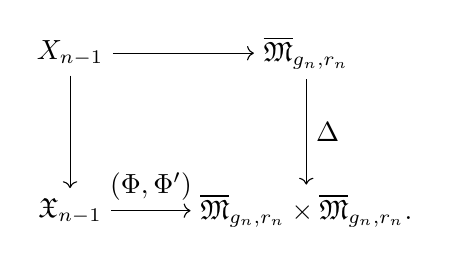
\begin{tikzpicture}[auto]
      \node (X) at (0, 2) {$X_{n - 1}$};
      \node (mX) at (0, 0) {$\model{X}_{n - 1}$};
      \node (M) at (3, 2) {$\Mbar{g_n}{r_n}$};
      \node (MM) at (3, 0) {$\Mbar{g_n}{r_n} \times \Mbar{g_n}{r_n}$.};
      \draw[->] (X) to node {} (mX);
      \draw[->] (X) to node {} (M);
      \draw[->] (M) to node {$\diagonal$} (MM);
      \draw[->] (mX) to node {$(\Phi, \Phi')$} (MM);
    \end{tikzpicture}
  \end{center}
  Note that $\diagonal$ is finite (and unramified) morphism since $\Mbar{g_n}{r_n}$ is separated and Deligne-Mumford algebraic stack, and the fiber product $\model{X}_{n - 1} \times_{\Mbar{g_n}{r_n} \times \Mbar{g_n}{r_n}} \Mbar{g_n}{r_n}$ is just the $\mathrm{Isom}$-scheme $\mathrm{Isom}_{\model{X}_{n - 1}}(\model{X}_n, \model{X}'_n)$, which is representable by a scheme. Since $\model{X}_{n - 1}$ is normal by Lemma \ref{NormalityOfStableCompactification}, it follows that the morphism $(\Phi, \Phi') \colon \model{X}_{n - 1} \to \Mbar{g_n}{r_n} \times \Mbar{g_n}{r_n}$ factors through $\diagonal$; in particular, we obtain the equality $\Phi = \Phi'$. Therefore, by the definition involved, we obtain an isomorphism $\model{X}_n \cong \model{X}'_n$ over $\model{X}_{n - 1}$, which completes the proof of the lemma.
\end{proof}

\begin{defn}
  Let $K$ be a discrete valuation field and $X = X_n \to X_{n - 1} \to \cdots \to X_1 \to X_0 = \Spec \, K$ a hyperbolic polycurve over $K$. Assume that $X$ admits a compactified stable model $\model{X} = \model{X}_n \to \model{X}_{n - 1} \to \cdots \to \model{X}_1 \to \model{X}_0 = \Spec \, \mathcal{O}_K$ with respect to its parametrization.
  \begin{enumerate}
    \item Let $x \in \model{X}_n$ be a point. Write $x_i$ for the image of $x$ in $X_i$ for each $i = 0, \ldots, n$. We shall say that $x$ is a \emph{stratum point} of $\model{X}_n$ if the following condition is satisfied:
    \begin{itemize}
      \item for each $i = 1, \ldots, n$, the point $x_i$ is either a node of the stable curve $(\model{X}_i,  \model{D}_i) \times_{\model{X}_{i - 1}} x_{i - 1} \to x_{i - 1}$, a marked point of the stable curve $(\model{X}_i, \model{D}_i) \times_{\model{X}_{i - 1}} x_{i - 1} \to x_{i - 1}$, or a generic point of an irreducible component of the stable curve $(\model{X}_i, \model{D}_i) \times_{\model{X}_{i - 1}} x_{i - 1} \to x_{i - 1}$. 
    \end{itemize}
    \item Let $x$ be a stratum point of $\model{X}_n$. Let $x_i$ be the image of $x$ in $\model{X}_i$ for each $i = 0, \ldots, n$. We shall say that the \emph{VCNGS-signature} of $x$ is the function $\sign{x} \colon \{1, \ldots, n\} \to \{\textV, \textC, \textN, \textG, \textS\}$ defined as follows:
    \begin{itemize}
      \item for each $i = 1, \ldots, n$, $\sign{x}(i) = \textV$ if $x_i$ is a generic point of an irreducible component of the stable curve $(\model{X}_i, \model{D}_i) \times_{\model{X}_{i - 1}} x_{i - 1} \to x_{i - 1}$;
      \item for each $i = 1, \ldots, n$, $\sign{x}(i) = \textC$ if $x_i$ is a marked point of the stable curve $(\model{X}_i, \model{D}_i) \times_{\model{X}_{i - 1}} x_{i - 1} \to x_{i - 1}$;
      \item for each $i = 1, \ldots, n$, $\sign{x}(i) = \textN$ if $x_i$ is a node of the stable curve $(\model{X}_i, \model{D}_i) \times_{\model{X}_{i - 1}} x_{i - 1} \to x_{i - 1}$;
      \item for $i = 0$, $\sign{x}(i) = \textG$ if $x_i$ is the generic point of $\Spec \, \mathcal{O}_K$;
      \item for $i = 0$, $\sign{x}(i) = \textS$ if $x_i$ is the closed point of $\Spec \, \mathcal{O}_K$.
    \end{itemize}
  \item Let $x$ be a stratum point of $\model{X}_n$. We shall say that the \emph{combinatorial dimension} of $x$ is the number of $i \in \{0, \ldots, n\}$ such that $\sign{x}(i) \in \{\textV, \textG\}$.
  \end{enumerate}
\end{defn}

\begin{lem}[Stratification of the stable compactification]\label{StratificationOfStableCompactification}
  Let $K$ be a discrete valuation field and $X = X_n \to X_{n - 1} \to \cdots \to X_1 \to X_0 = \Spec \, K$ a hyperbolic polycurve over $K$. Assume that $X$ admits a compactified stable model $\model{X} = \model{X}_n \to \model{X}_{n - 1} \to \cdots \to \model{X}_1 \to \model{X}_0 = \Spec \, \mathcal{O}_K$ with respect to its parametrization. Then there exists a stratification of $\model{X}_n$ such that
  \begin{itemize}
    \item the strata of the stratification are irreducible;
    \item the set of stratum points of $\model{X}_n$ coincides with the set of generic points of the strata of the stratification.
  \end{itemize}
  The stratification of $\model{X}_n$ is uniquely determined by the above conditions. Moreover, for each stratum $A$ of the stratification associated to $\model{X}_n$, the image of $A$ in $\model{X}_i$ is one of the strata of the stratification associated to $\model{X}_i$ for each $i = 0, \ldots, n - 1$.
\end{lem}
\begin{proof}
  First, we shall construct a stratification of $\model{X}_n$ by induction on the relative dimension $n$ of $X$ over $\Spec \, K$. The case where $n = 0$ is trivial, so we assume that $n > 0$ and that the lemma holds for any hyperbolic polycurve of relative dimension less than $n$.

  Let $\pi$ be the morphism $\model{X}_n \to \model{X}_{n - 1}$. For each strata $A$ of the stratification of $\model{X}_{n - 1}$ obtained by the induction hypothesis, we shall construct a decomposition of $\pi^{-1}(A)$ by locally closed subsets as follows. Let $\eta_A$ be the generic point of $A$. Then the set of stratum points over $\eta_A$ coincides with the set of nodes, marked points, and generic points of irreducible components of the stable curve $(\model{X}_n, \model{D}_n) \times_{\model{X}_{n - 1}} \eta_A \to \eta_A$. For the stratum points $s$ over $\eta_A$ which are nodes or marked points of the stable curve $(\model{X}_n, \model{D}_n) \times_{\model{X}_{n - 1}} \eta_A \to \eta_A$, we define the subscheme $B_s$ to be the closure of $s$ in $\pi^{-1}(A)$. For the stratum points $t$ over $\eta_A$ which are generic points of irreducible components of the stable curve $(\model{X}_n, \model{D}_n) \times_{\model{X}_{n - 1}} \eta_A \to \eta_A$, we define the subscheme $B_t$ as follows: let $s_1, \ldots, s_m$ be the nodes and marked points of the stable curve $(\model{X}_n, \model{D}_n) \times_{\model{X}_{n - 1}} \eta_A \to \eta_A$ which are contained in the irreducible component corresponding to $t$, and let $B_{s_1}, \ldots, B_{s_m}$ be the strata defined above corresponding to $s_1, \ldots, s_m$. Then we define $B_t$ to be the complement of $\bigcup_{i = 1}^m B_{s_i}$ in the closure of $t$ in $\pi^{-1}(A)$.

  Let $t_1, \ldots, t_l$ be the stratum points of $\model{X}_n$ over $\eta_A$ which are generic points of irreducible components of the stable curve $(\model{X}_n, \model{D}_n) \times_{\model{X}_{n - 1}} \eta_A \to \eta_A$, and let $s_1, \ldots, s_m$ be the stratum points of $\model{X}_n$ over $\eta_A$ which are nodes or marked points of the stable curve $(\model{X}_n, \model{D}_n) \times_{\model{X}_{n - 1}} \eta_A \to \eta_A$. Note that it follows immediately from the construction and induction hypothesis that the strata $B_{t_1}, \ldots, B_{t_l}, B_{s_1}, \ldots, B_{s_m}$ are irreducible, locally closed in $\model{X}_n$, and mutually disjoint. Moreover, by the going-down theorem, every point of $\pi^{-1}(A)$ has a generalization which is a stratum point over $\eta_A$. Therefore, $B_{t_1}, \ldots, B_{t_l}, B_{s_1}, \ldots, B_{s_m}$ constitute a decomposition of $\pi^{-1}(A)$ by locally closed subsets. Since every stratum point of $\model{X}_n$ is over a stratum point of $\model{X}_{n - 1}$, it follows that the decompositions obtained by performing the above construction for all strata of $\model{X}_{n - 1}$ constitute a decomposition of $\model{X}_n$ such that the set of stratum points of $\model{X}_n$ coincides with the set of generic points of the strata of the decomposition.

  Finally, since the closure of a stratum point $x_n$ of $\model{X}_n$ is either a finite \'{e}tale cover over the closure of the image $x_{n - 1}$ or an underlying scheme of a stable curve over the closure of the image $x_{n - 1}$ of $x_n$ in $\model{X}_{n - 1}$, it follows from the induction hypothesis and the various definitons involved that the above decomposition of $\model{X}_n$ is indeed a stratification.

  The remaining assertions of the lemma follow immediately from the construction and the definitions involved. This completes the proof of the lemma.
\end{proof}

\begin{lem}[Dimension of strata of the stable compactification]\label{DimensionOfStrataOfStableCompactification}
  Let $K$ be a complete discrete valuation field and $X = X_n \to X_{n - 1} \to \cdots \to X_1 \to X_0 = \Spec \, K$ a hyperbolic polycurve over $K$. Assume that $X$ admits a compactified stable model $\model{X} = \model{X}_n \to \model{X}_{n - 1} \to \cdots \to \model{X}_1 \to \model{X}_0 = \Spec \, \mathcal{O}_K$ with respect to its parametrization. Let $\mathfrak{A}$ be the stratification of $\model{X}_n$ obtained by applying the construction in Lemma \ref{StratificationOfStableCompactification} to the hyperbolic polycurve $X_n$. Then for each stratum $A$ of $\mathfrak{A}$, the dimension of the closure of $A$ in $\model{X}_n$ coincides with the combinatorial dimension of the stratum points corresponding to the stratum $A$.
\end{lem}
\begin{proof}
  By noting that $\mathcal{O}_K$ is excellent (in particular, universally catenary), it follows immediately from the elementary scheme theory and the various definitions involved.
\end{proof}

\begin{lem}[Strata of codimension $0$ and $1$ of the stable compactification]\label{StrataOfCodimensionZeroAndOne}
  Let $K$ be a discrete valuation field and $X = X_n \to X_{n - 1} \to \cdots \to X_1 \to X_0 = \Spec \, K$ a hyperbolic polycurve over $K$. Assume that $X$ admits a compactified stable model $\model{X} = \model{X}_n \to \model{X}_{n - 1} \to \cdots \to \model{X}_1 \to \model{X}_0 = \Spec \, \mathcal{O}_K$ with respect to its parametrization. Let $\mathfrak{A}$ be the stratification of $\model{X}_n$ obtained by applying the construction in Lemma \ref{StratificationOfStableCompactification} to the hyperbolic polycurve $X_n$.
  \begin{enumerate}
    \item Let $x$ be a stratum point of $\model{X}_n$, and let $d_x$ be the combinatorial dimension of $x$. Then the following conditions are equivalent:
      \begin{enumerate}
        \item $d_x = n + 1$;
        \item the stratum point $x$ is a generic point of $\model{X}_n$.
      \end{enumerate}
    Moreover, if the above conditions are satisfied, the corresponding stratum coincides with $X_n$ as a subscheme of $\model{X}_n$.
    \item Let $x$ be a stratum point of $\model{X}_n$, and let $d_x$ be the combinatorial dimension of $x$. Then the following conditions are equivalent:
      \begin{enumerate}
        \item $d_x = n$;
        \item the stratum point $x$ is a generic point of an irreducible component of the divisor at infinity of $\model{X}_n$, i.e., a generic point of an irreducible component of the closed subspace $\model{X}_n \setminus X_n$ of $\model{X}_n$.
      \end{enumerate}
    Moreover, for every irreducible component $D$ of the divisor at infinity of $\model{X}_n$, the generic point of $D$ is a stratum point of $\model{X}_n$.
  \end{enumerate}
\end{lem}
\begin{proof}
It follows immediately from the definitions involved.
\end{proof}

\begin{defn}
  Let $K$ be a discrete valuation field and $X = X_n \to X_{n - 1} \to \cdots \to X_1 \to X_0 = \Spec \, K$ a hyperbolic polycurve over $K$. Assume that $X$ admits a compactified stable model $\model{X} = \model{X}_n \to \model{X}_{n - 1} \to \cdots \to \model{X}_1 \to \model{X}_0 = \Spec \, \mathcal{O}_K$ with respect to its parametrization. Let $\mathfrak{A}$ be the stratification of $\model{X}_n$ obtained by applying the construction in Lemma \ref{StratificationOfStableCompactification} to the hyperbolic polycurve $X_n$.
  \begin{enumerate}
    \item We shall say that an irreducible component $D$ of the divisor at infinity of $\model{X}_n$, i.e., an irreducible component of the closed subspace $\model{X}_n \setminus X_n$ of $\model{X}_n$, is a \emph{divisor of cusp-type} if the following condition is satisfied:
    \begin{itemize}
      \item there exists an element $i \in \{1, \ldots, n\}$ such that $\sign{\eta_D}(i) = \textC$, where $\eta_D$ is the generic point of $D$.
    \end{itemize}
    Moreover, we shall say that the number of $i \in \{1, \ldots, n\}$ such that $\sign{\eta_D}(i) = \textC$ is the \emph{C-level} of $D$.
    \item We shall say that an irreducible component $D$ of the divisor at infinity of $\model{X}_n$, i.e., an irreducible component of the closed subspace $\model{X}_n \setminus X_n$ of $\model{X}_n$, is a \emph{divisor of vertex-type} if the following condition is satisfied:
    \begin{itemize}
      \item for every $i \in \{1, \ldots, n\}$, $\sign{\eta_D}(i) = \textV$, where $\eta_D$ is the generic point of $D$.
    \end{itemize}
  \end{enumerate}
\end{defn}

\begin{lem}[Strata and Divisors of Infinity of the stable compactification]\label{StrataAndDivisorsOfInfinityOfStableCompactification}
  Let $K$ be a discrete valuation field and $X = X_n \to X_{n - 1} \to \cdots \to X_1 \to X_0 = \Spec \, K$ a hyperbolic polycurve over $K$. Assume that $X$ admits a compactified stable model $\model{X} = \model{X}_n \to \model{X}_{n - 1} \to \cdots \to \model{X}_1 \to \model{X}_0 = \Spec \, \mathcal{O}_K$ with respect to its parametrization. Let $\mathfrak{A}$ be the stratification of $\model{X}_n$ obtained by applying the construction in Lemma \ref{StratificationOfStableCompactification} to the hyperbolic polycurve $X_n$. Then for each stratum $A$ of $\mathfrak{A}$ and each irreducible component of the divisor at infinity $D$ of $\model{X}_n$, i.e., each irreducible component of the closed subspace $\model{X}_n \setminus X_n$ of $\model{X}_n$, $A$ is either contained in $D$ or disjoint from $D$.
\end{lem}
\begin{proof}
  By the construction of the stratification of $\model{X}_n$, which is given in the proof of Lemma \ref{StratificationOfStableCompactification}, it follows immediately that the divisor $D$ is a disjoint union of strata of the stratification of $\model{X}_n$. Therefore, for each stratum $A$ of the stratification of $\model{X}_n$, the intersection $A \cap D$ is either empty or coincides with $A$. This completes the proof of the lemma.
\end{proof}

\begin{lem}[Strata and Divisors of Infinity of the moduli stack of stable curves]\label{StrataAndDivisorsOfInfinityOfModuliStack}
  Let $K$ be a discrete valuation field and $X = X_n \to X_{n - 1} \to \cdots \to X_1 \to X_0 = \Spec \, K$ a hyperbolic polycurve over $K$. Assume that $X$ admits a compactified stable model $\model{X} = \model{X}_n \to \model{X}_{n - 1} \to \cdots \to \model{X}_1 \to \model{X}_0 = \Spec \, \mathcal{O}_K$ with respect to its parametrization. Let $\mathfrak{A}$ be the stratification of $\model{X}_{n - 1}$ obtained by applying the construction in Lemma \ref{StratificationOfStableCompactification} to the hyperbolic polycurve $X_{n - 1}$, and let $\varPhi \colon \model{X}_{n - 1} \to \Mbar{g_n}{r_n}$ be the morphism determined by the stable curve $(\model{X}_n, \model{D}_n) \to \model{X}_{n - 1}$. Then for each stratum $A$ of $\mathfrak{A}$ and each irreducible component of the divisor at infinity $D$ of the moduli stack $\Mbar{g_n}{r_n}$, i.e., each irreducible component of the boundary $\Mbar{g_n}{r_n} \setminus \M{g_n}{r_n}$, the intersection $\varPhi^{-1}(D) \cap A$ is either empty or coincides with $A$.
\end{lem}
\begin{proof}
  By noting that $\Mbar{g_n}{r_n}$ is a smooth Deligne-Mumford algebraic stack over $\Spec \, \mathbb{Z}$, it follows that for each divisor of $\Mbar{g_n}{r_n}$, the pullback of the divisor to $\model{X}_{n - 1}$ is a Cartier divisor. Thus, the assertion follows formally from the Lemma \ref{StrataAndDivisorsOfInfinityOfStableCompactification}. This completes the proof of the lemma.
\end{proof}   

% #endregion

% #region Generalities on \'etale locally log-constant fs log schemes

\begin{defn}
  Let $X^\log$ be a locally Noetherian fs log scheme.
  \begin{enumerate}
    \item We shall say that $X^\log$ is \emph{log-constant}, if there exists an fs monoid $P$ and the chart $\underline{P} \to \mathcal{M}_{X^\log}$ of the log structure $\mathcal{M}_{X^\log}$ on $X$ such that the induced morphism $\underline{P} \to \mathcal{C}_{X^\log}$ (where $\underline{P}$ is the constant sheaf associated to $P$) is an isomorphism. We shall refer to such a monoid $P$ as a \emph{type} of $X^\log$, and we shall say that $X^\log$ is of type $P$.
    \item We shall say that $X^\log$ is \emph{\'{e}tale locally log-constant} at $x \in X$, if there exists an \'{e}tale neighborhood $U$ of $x$ such that the restriction of $X^\log$ to $U$ is log-constant. We shall say that $X^\log$ is \emph{\'{e}tale locally log-constant}, if $X^\log$ is \'{e}tale locally log-constant at every point of $X$. For each connected component of $X$, we shall say that a monoid $P$ is a \emph{type} of $X^\log$ at the connected component if there exists an \'{e}tale covering $U$ of the connected component such that the restriction of $X^\log$ to $U$ is log-constant of type $P$. If $X$ is connected, we shall simply say that $P$ is a type of $X^\log$.
    \item We shall say that $X^\log$ is \emph{characteristic-constant}, if the \'{e}tale sheaf of characteristic $\mathcal{C}_{X^\log}$ of $X^\log$ is a constant sheaf. Let $P$ be a monoid. Then we shall refer to an isomorphism $\underline{P} \cong \mathcal{C}_{X^\log}$ as a \emph{trivialization of characteristic} of $X^\log$ (of type $P$).
    \item Let $X^\log$ be an \'{e}tale locally log-constant fs log scheme. Let $n$ be an integer. Then we shall say that $X^\log$ is of \emph{log-rank} $n$ if there exists an fs monoid $P$ such that $X^\log$ is of type $P$ and the rank of $P^\gp$ is equal to $n$.
  \end{enumerate}
\end{defn}

\begin{rem}
  The above definitions are an immediate generalization of the notion of ``a morphism of type $\Nat^{\oplus n}$", which is introduced in \cite{Hoshi1}.
\end{rem}

\begin{rem}
  We can easily generalize the above definitions to the relative situation, i.e., for a morphism of fs log schemes $f \colon X^\log \to Y^\log$ whose underlying morphism of schemes is an isomorphism, we can define the notions of $f$ being log-constant, \'etale locally log-constant, or characteristic-constant by replacing $\mathcal{C}_{X^\log}$ with the \'{e}tale sheaf of relative characteristic $\mathcal{C}_{X^\log/Y^\log}$ of $f$ in the above definitions. However, we shall not need such a generalization in this paper, and therefore we do not give a precise definition of these notions.
\end{rem}

\begin{lem}[Characterization of \'{e}tale locally log-constant fs log schemes]\label{CharacterizationOfEtaleLocallyLogConstantLogSchemes}
  Let $X^\log$ be an fs log scheme. Then the following conditions are equivalent:
  \begin{enumerate}
    \item $X^\log$ is \'{e}tale locally log-constant;
    \item the \'{e}tale sheaf of characteristic $\mathcal{C}_{X^\log}$ of $X^\log$ is \'{e}tale locally constant.
  \end{enumerate}
\end{lem}
\begin{proof}
  It follows immediately from the definitions involved.
\end{proof}

\begin{lem}[Correspondence between characteristic-constant log schemes and certain homomorphisms to the Picard group]\label{CharacteristicConstantLogSchemes}
  Let $X$ be a reduced scheme and $P$ be an fs sharp monoid. Write $\mathbf{M}_X$ for the set of isomorphism classes of pairs $(\mathcal{M}, \alpha)$ such that
  \begin{itemize}
    \item $\mathcal{M}$ is an fs log structure on $X$;
    \item Let $X^\log$ be the fs log scheme whose underlying scheme is $X$ and whose log structure is $\mathcal{M}$. Then $X^\log$ is characteristic-constant and of type $P$;
    \item $\alpha \colon \underline{P} \to \mathcal{C}_{(X, \mathcal{M})}$ is an isomorphism.
  \end{itemize}
  Write $\iota_X \colon \mathbf{M}_X \to \mathrm{Hom}(P, \mathrm{Pic}(X)) = \mathrm{Hom}(P^\gp, \mathrm{Pic}(X))$ for the map defined as follows:
  \begin{itemize}
    \item For each element $(\mathcal{M}, \alpha)$ of $\mathbf{M}_X$, write $X^\log$ for the fs log scheme whose underlying scheme is $X$ and whose log structure is $\mathcal{M}$. Then we define $\iota_X(\mathcal{M}, \alpha)$ to be the homomorphism $P \to \mathrm{Pic}(X)$ defined as follows: for each element $p$ of $P$, we define $\iota_X(\mathcal{M}, \alpha)(p)$ to be the isomorphism class of the invertible sheaf $(\alpha \circ \mathrm{pr})^{-1}(p)$ on $X$, where $\mathrm{pr} \colon \mathcal{M}_{X^\log} \to \mathcal{C}_{X^\log}$ is the natural projection.
  \end{itemize}
  Then the map $\iota_X$ is a bijection.
\end{lem}
\begin{proof}
  First, we shall construct the (inverse) map $\kappa_X \colon \mathrm{Hom}(P, \mathrm{Pic}(X)) \to \mathbf{M}_X$ of $\iota_X$. Let $f \colon P \to \mathrm{Pic}(X)$ be a homomorphism. Write $f^\gp \colon P^\gp \to \mathrm{Pic}(X)$ for the homomorphism induced by $f$ on the groupifications. Temporarily, we take an isomorphism $v \colon \Int^{\oplus n} \to P^\gp$ of abelian groups, where $n$ is the rank of $P^\gp$. For $1 \leq i \leq n$, we write $\mathbf{e}_i$ for the $i$-th standard basis vector of $\Int^{\oplus n}$. Write $\mathcal{L}_i$ for the invertible sheaf on $X$ corresponding to $f^\gp(v(\mathbf{e}_i))$. Then we define an extension $0 \to \mathcal{O}_X^\times \to \mathcal{M} \to \underline{P} \to 0$ of sheaves on $X$ as follows: we define $\mathcal{M}$ to be the coproduct of $\mathcal{L}_1^{\otimes a_1} \otimes \cdots \otimes \mathcal{L}_n^{\otimes a_n}$ for all $a_1, \ldots, a_n \in \Int$ such that $v(a_1 \mathbf{e}_1 + \cdots + a_n \mathbf{e}_n) \in P$ as a sheaf of sets, and we define the monoid structure on $\mathcal{M}$ by the natural (various) isomorphisms. This construction yields an bijective correspondence between the set of extensions of $\underline{P}$ by $\mathcal{O}_X^\times$ and the set of homomorphisms from $P$ to $\mathrm{Pic}(X)$. Next, we shall construct a log structure $\mathcal{M} \to \mathcal{O}_X$ on $X$. Let $s$ be a local section of $\mathcal{M}$, and let $p$ be an element of $P$ such that the image of $s$ in $\underline{P}$ is coincides with $p$. Then we define the image of $s$ of the morphism $\mathcal{M} \to \mathcal{O}_X$ to be $s$ ($\in \mathcal{O}_X^\times$) if $p = 0$ and to be $0$ if $p \neq 0$. This construction yields a log structure on $X$, and the resulting fs log scheme is characteristic-constant and of type $P$. Thus, we have constructed the map $\kappa_X \colon \mathrm{Hom}(P, \mathrm{Pic}(X)) \to \mathbf{M}_X$.

  Finally, we verify that $\iota_X$ and $\kappa_X$ are inverse to each other. For each element $(\mathcal{M}, \alpha)$ of $\mathbf{M}_X$, we have an extension $0 \to \mathcal{O}_X^\times \to \mathcal{M} \to \underline{P} \to 0$ of sheaves on $X$, and the corresponding homomorphism $P \to \mathrm{Pic}(X)$. To verify the assertion that $\iota_X$ and $\kappa_X$ are inverse to each other, it suffices to verify that the log structure $\mathcal{M} \to \mathcal{O}_X$ satisfies the following condition: for each local section $s$ of $\mathcal{M}$ and each element $p$ of $P$ such that the image of $s$ in $\underline{P}$ coincides with $p$, the image of $s$ by the morphism $\mathcal{M} \to \mathcal{O}_X$ coincides with $s$ if $p = 0$ and with $0$ if $p \neq 0$. The case $p = 0$ is trivial, so we assume that $p \neq 0$. Since the condition is local, we can check it on a smaller open subset.

  Let $U$ be an \'{e}tale open subset of $X$ such that $s$ is defined, and the (local) chart $\varphi \colon \underline{P}_U \to \mathcal{M}|_U$ of the log structure $\mathcal{M}$ on $X$ exists. Then $s$ can be written as $\varphi(p) \cdot u$ for some $u \in \mathcal{O}_X^\times(U)$. Since the image of $\varphi(p)$ in $\mathcal{C}$ is nonzero everywhere on $U$, where $\mathcal{C}$ is the \'{e}tale sheaf of characteristic of $\mathcal{M}$, it follows that the image of $\varphi(p)$ by the morphism $\mathcal{M} \to \mathcal{O}_X$ is not invertible at every point of $U$. Therefore, since $X$ is reduced, the image of $\varphi(p)$ by the morphism $\mathcal{M} \to \mathcal{O}_X$ is $0$. This completes the verification that $\iota_X$ and $\kappa_X$ are inverse to each other, and therefore completes the proof of the lemma.
\end{proof}

\begin{defn}
  Let $X$ be a reduced scheme and $P$ be an fs sharp monoid. Let $(X^\log, \alpha)$ be a pair consisting of an fs log scheme $X^\log$ whose underlying scheme is $X$ and an isomorphism $\alpha \colon \underline{P} \to \mathcal{C}_{X^\log}$. Let $f \colon P \to \mathrm{Pic}(X)$ be the homomorphism corresponding to $(X^\log, \alpha)$ via the bijection $\iota_X$ in Lemma \ref{CharacteristicConstantLogSchemes}. We shall say that the pair $(X^\log, \alpha)$ is associated to the homomorphism $f$.
\end{defn}

\begin{lem}[Description of the log structure of the stable compactification]\label{DescriptionOfLogStructureOfStableCompactification}
  Let $K$ be a discrete valuation field and $X = X_n \to X_{n - 1} \to \cdots \to X_1 \to X_0 = \Spec \, K$ a hyperbolic polycurve over $K$. Assume that $X$ admits a compactified stable model $\model{X} = \model{X}_n \to \model{X}_{n - 1} \to \cdots \to \model{X}_1 \to \model{X}_0 = \Spec \, \mathcal{O}_K$ with respect to its parametrization. Let $\mathfrak{A}$ be the stratification of $\model{X}_n$ obtained by applying the construction in Lemma \ref{StratificationOfStableCompactification} to the hyperbolic polycurve $X_n$. Let $A$ be a stratum of $\mathfrak{A}$. Then the following assertions hold:
  \begin{enumerate}
    \item Write $A^\log$ for the fs log scheme whose underlying scheme is $A$, endowed with the reduced scheme structure, and whose log structure is the pullback of the log structure on $\model{X}_n^\log$. Then $A^\log$ is \'{e}tale locally log-constant.
    \item Let $\eta_A$ be the generic point of $A$. Let $\pi$ be the morphism $\model{X}_n \to \model{X}_{n - 1}$, and let $\overline{A}$ be the image of $A$ in $\model{X}_{n - 1}$ by $\pi$. Let $\eta_{\overline{A}}$ be the generic point of $\overline{A}$. We note that $\eta_A$ and $\eta_{\overline{A}}$ are stratum points of $\model{X}_n$ and $\model{X}_{n - 1}$, respectively. Define $A^\log$, $\overline{A}^\log$ for the fs log schemes as in (i) above. Then the following assertions hold:
      \begin{enumerate}
        \item If $\sign{\eta_A}(n) = \textV$, then the morphism $A^\log \to \overline{A}^\log$ induced by $\pi$ is strict, i.e., the type of $A^\log$ coincides with the type of $\overline{A}^\log$.
        \item If $\sign{\eta_A}(n) = \textC$, then there exists a natural isomorphism $\mathcal{C}_{A^\log} \cong \mathcal{C}_{\overline{A}^\log}|_A \oplus \underline{\Nat}$ of \'{e}tale sheaves on $A$, where $\underline{\Nat}$ is the constant sheaf associated to $\Nat$.
        \item Let $P$ be the type of $A^\log$ and $\overline{P}$ be the type of $\overline{A}^\log$. If $\sign{\eta_A}(n) = \textN$, then there exists a pushout diagram of monoids:
        \begin{center}
          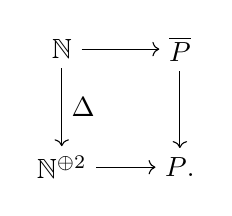
\begin{tikzpicture}[auto]
          \node (N) at (0, 1.5) {$\Nat$};
          \node (N2) at (0, 0) {$\Nat^{\oplus 2}$};
          \node (Pbar) at (1.5, 1.5) {$\overline{P}$};
          \node (P) at (1.5, 0) {$P$.};
          \draw[->] (N) to node {} (Pbar);
          \draw[->] (N2) to node {} (P);
          \draw[->] (N) to node {$\diagonal$} (N2);
          \draw[->] (Pbar) to node {} (P);
          \end{tikzpicture}
        \end{center}
      \end{enumerate}
    \item Let $\eta_A$ be the generic point of $A$, and let $d_A$ be the combinatorial dimension of $\eta_A$. Then the log rank of $A^\log$ is equal to $n + 1 - d_A$.
  \end{enumerate}
\end{lem}
\begin{proof}
  In light of Lemma \ref{StrataAndDivisorsOfInfinityOfModuliStack}, it follows immediately from the description of the (log) structure of the stable curves (cf. \cite{KatoF}) and the various definitions involved.
\end{proof}

\begin{lem}[Finiteness of automorphism groups of fs sharp monoids]\label{FinitenessOfAutomorphismGroupsOfSharpMonoids}
  Let $P$ be an fs sharp monoid. Then the automorphism group $\Aut(P)$ of $P$ is finite.
\end{lem}
\begin{proof}
  It follows from the well-known fact that the set of irreducible elements of $P$, i.e., the set of nonzero elements of $P$ which cannot be written as a sum of two nonzero elements of $P$, is finite and generates $P$ as a monoid, that the automorphism group $\Aut(P)$ of $P$ is finite. This completes the proof of the lemma.
\end{proof}

\begin{lem}[Representability of the functor of trivializations of characteristic of \'{e}tale locally log-constant fs log schemes]\label{RepresentabilityOfFunctorOfTrivializationsOfCharacteristicOfEtaleLocallyLogConstantLogSchemes}
  Let $X^\log$ be a locally Noetherian, connected fs log scheme which is \'{e}tale locally log-constant. Let $P$ be a monoid which is a type of $X^\log$. Define a functor $F_{X, P}$ from the category of schemes $\mathsf{Sch}$ to the category of sets $\mathsf{Set}$ as follows: for each scheme $S$, we define $F_{X, P}(S)$ to be the set of pairs $(f, \alpha)$ such that
  \begin{itemize}
    \item the morphism of schemes $f \colon S \to X$;
    \item the isomorphism $\alpha \colon \underline{P} \to f^*\mathcal{C}_{X^\log}$.
  \end{itemize}
  Then the functor $F_{X, P}$ is representable by a scheme, and the (canonical) morphism $F_{X, P} \to X$ is a finite \'{e}tale covering.
\end{lem}
\begin{proof}
  Take an \'{e}tale covering $U$ of $X$ such that the pullback of $\mathcal{C}_{X^\log}$ is a constant sheaf. Write $F_1$ for the scheme \[\coprod_{V \subset U \, : \, \text{conn. comp.}} \coprod_{f \in \mathrm{Hom}(\underline{P}_V, \mathcal{C}_{X^\log}|_V)} V. \]

  In light of the general theory of descent, and since $\Aut(P)$ is finite by Lemma \ref{FinitenessOfAutomorphismGroupsOfSharpMonoids}, it follows that the scheme $F_1$ naturally descends to a scheme $F_0$ which is finite \'{e}tale over $X$, and $F_0$ represents the functor $F_{X, P}$. This completes the proof of the lemma.
\end{proof}

\begin{thm}[Exact sequence of log fundamental groups of fs log schemes which are \'{e}tale locally log-constant]\label{ExactSequenceOfLogFundamentalGroupsOfEtaleLocallyLogConstantLogSchemes}
  Let $X^\log$ be a connected, reduced fs log scheme which is \'{e}tale locally log-constant. Write $X$ for the underlying scheme of $X^\log$, or the log scheme obtained by endowing $X$ with the trivial log structure. Let $x$ be a geometric point of $X$, and let $\tilde{x}$ be a log geometric point of $X^\log$ lying over $x$. Then there exists an exact sequence of profinite groups
  \[
    \pi_1(X^\log \times_X x, \tilde{x}) \to \pi_1(X^\log, \tilde{x}) \to \pi_1(X, x) \to 1.
  \]
\end{thm}
\begin{proof}
  First, we observe that we may assume without loss of generality that $X$ is characteristic-constant. Indeed, by Lemma \ref{RepresentabilityOfFunctorOfTrivializationsOfCharacteristicOfEtaleLocallyLogConstantLogSchemes}, there exists a connected finite \'{e}tale covering $Y$ of $X$ such that the pullback of $\mathcal{C}_{X^\log}$ to $Y$ is a constant sheaf. Write $Y^\log$ for the fs log scheme whose underlying scheme is $Y$ and whose log structure is the pullback of the log structure on $X^\log$. Then $Y^\log$ is characteristic-constant. Now we observe that there exists a pullback diagram of profinite groups:
  \begin{center}
    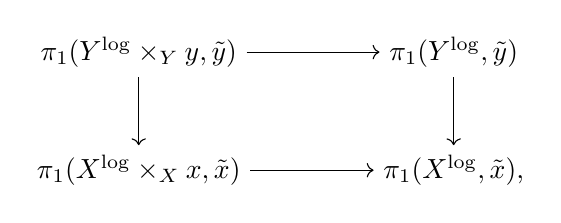
\begin{tikzpicture}[auto]
    \node (A) at (0, 1.5) {$\pi_1(Y^\log \times_Y y, \tilde{y})$};
    \node (B) at (0, 0) {$\pi_1(X^\log \times_X x, \tilde{x})$};
    \node (C) at (4, 1.5) {$\pi_1(Y^\log, \tilde{y})$};
    \node (D) at (4, 0) {$\pi_1(X^\log, \tilde{x})$,};
    \draw[->] (A) to node {} (B);
    \draw[->] (C) to node {} (D);
    \draw[->] (A) to node {} (C);
    \draw[->] (B) to node {} (D);
    \end{tikzpicture}
  \end{center}
  for some geometric point $y$ of $Y$ lying over $x$ and some log geometric point $\tilde{y}$ of $Y^\log$ lying over $y$. Thus, if we verify the exactness of the sequence in the assertion for $Y^\log$, then it follows that the sequence in the assertion is also exact for $X^\log$. Therefore, we may assume without loss of generality that $X$ is characteristic-constant.

  Next, we observe that we may assume without loss of generality that $\Nat^{\oplus n}$ is the type of $X^\log$ for some integer $n$. Indeed, by the elementary monoid theory, there exists an injection $P \to \Nat^{\oplus n}$ of monoids for some integer $n$, which induces an isomorphism $P^\gp \cong (\Nat^{\oplus n})^\gp$. By the description of characteristic-constant log schemes, stated in Lemma \ref{CharacteristicConstantLogSchemes}, it follows that there exists a morphism $X'^\log \to X^\log$ of fs log schemes such that the underlying morphism of schemes is an isomorphism and induced morphism on the characteristic is isomorphic (as a morphism of monoid sheaves) to the injection $\underline{P} \to \underline{\Nat^{\oplus n}}$.

  We now proceed to show that the (natural) morphism of Galois categories $\mathrm{F\acute{e}t}(X^\log) \to \mathrm{F\acute{e}t}(X'^\log)$ is an equivalence. By the descent theory of log schemes (cf. \cite[Proposition 4.4]{Vidal}, \cite[Proposition B.8]{Hoshi1}), it suffices to verify the case where $X$ is the spectrum of a strictly henselian local ring. However, the assertion follows immediately from the description of the k\'{e}t covering of a strictly henselian local fs log scheme (cf. \cite[Proposition B.2]{Hoshi1}).

  Finally, we verify the exactness of the sequence in the assertion for $X^\log$ such that $\Nat^{\oplus n}$ is the type of $X^\log$ for some integer $n$. However, it follows immediately from \cite[Corollary 2]{Hoshi1}.
\end{proof}

% #endregion

% #region Pro-$\ell$-exactness and graphical inertness of hyperbolic polycurves, pro-$\ell$ decomposition groups and inertia groups

% #region working
\begin{lem}[Slimness of the extension group of slim groups]\label{SlimnessOfExtensionGroupOfSlimGroups}
  Let $1 \to N \to G \to Q \to 1$ be an exact sequence of profinite groups. Assume that $N$ and $Q$ are slim. Then $G$ is also slim.
\end{lem}
\begin{proof}
  Let $H$ be an open subgroup of $G$. Let $g \in G$ be an element of centralizer of $H$. Then the image of $g$ in $Q$ is an element of the centralizer of the image of $H$ in $Q$, and therefore the image of $g$ in $Q$ is trivial. Thus, $g$ is an element of $N$. Since $g$ is an element of the centralizer of $H \cap N$ in $N$, together with the assumption that $N$ is slim, it follows that $g$ is trivial. This completes the proof of the lemma.
\end{proof}

\begin{defn}
  Let $K$ be a field, and let $X = X_n \to X_{n - 1} \to \cdots \to X_1 \to X_0 = \Spec \, K$ be a hyperbolic polycurve over $K$. Let $\ell$ be a prime number. We shall say that $X$ is \emph{geometrically pro-$\ell$-exact} if for each $0 \leq r < s < t \leq n$, then the sequence of profinite groups
    \[
      1 \to \GFG{X_t / X_s}^\ell \to \GFG{X_t / X_r}^\ell \to \GFG{X_s / X_r}^\ell \to 1
    \]
    is exact, where $\GFG{X_j / X_i}^\ell$ ($0 \leq i < j \leq n)$ is the maximal pro-$\ell$ quotient of the kernel of the morphism $\GFG{X_j} \to \GFG{X_i}$.
\end{defn}

\begin{lem}[Slimness of the geometric pro-$\ell$ fundamental group of a geometrically pro-$\ell$-exact hyperbolic polycurve]\label{SlimnessOfGeometricProEllFundamentalGroupOfGeometricallyProEllExactHyperbolicPolycurves}
  Let $K$ be a field, and let $X = X_n \to X_{n - 1} \to \cdots \to X_1 \to X_0 = \Spec \, K$ be a hyperbolic polycurve over $K$. Assume that $X$ is geometrically pro-$\ell$-exact. Then the geometric pro-$\ell$ fundamental group $\GFG{X}^\ell$ of $X$ is slim.
\end{lem}
\begin{proof}
  By Lemma \ref{SlimnessOfExtensionGroupOfSlimGroups} and induction on the (relative) dimension of the polycurve, and since the geometric pro-$\ell$ fundamental group of a hyperbolic curve is slim, the assertion follows immediately.
\end{proof}

\begin{lem}[Tameness of the outer representation of a geometrically pro-$\ell$-exact hyperbolic polycurve which admits a compactified stable model]\label{TamenessOfOuterRepresentationOfGeometricallyProEllExactHyperbolicPolycurvesAdmittingCompactifiedStableModels}
  Let $K$ be a complete discrete valuation field, and let $X = X_n \to X_{n - 1} \to \cdots \to X_1 \to X_0 = \Spec \, K$ be a hyperbolic polycurve over $K$. Let $\ell$ be a prime number which is invertible in $\mathcal{O}_K$. Assume $X$ admits a compactified stable model $\model{X} = \model{X}_n \to \model{X}_{n - 1} \to \cdots \to \model{X}_1 \to \model{X}_0 = \Spec \, \mathcal{O}_K$ with respect to its parametrization, and that $X$ is geometrically pro-$\ell$-exact. Then the outer representation $G_K \to \Out(\GFG{X}^\ell)$, which is induced by the exact sequence $1 \to \GFG{X}^\ell \to \GPRFG{\ell}{X} \to G_K \to 1$, factors through the profinite group $G_K/P_K$.
\end{lem}
\begin{proof}
  Let $s$ be the closed point of $\Spec \, \mathcal{O}_K$, and let $\overline{s}^\log$ be a log geometric point of $\Spec \, \mathcal{O}_K^\log$ lying over $s$. Consider the commutative diagram of homomorphisms of profinite groups:
  \begin{center}
    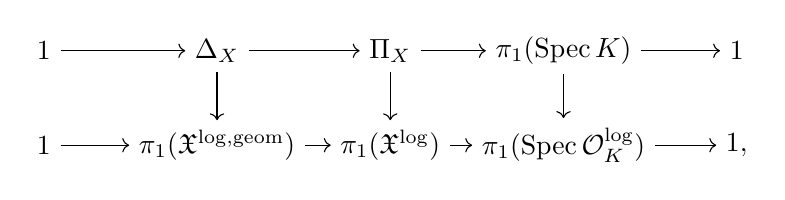
\begin{tikzpicture}[auto]
      \node (A) at (0, 1.2) {$1$};
      \node (B) at (0, 0) {$1$};
      \node (C) at (2.2, 1.2) {$\GFG{X}$};
      \node (D) at (2.2, 0) {$\pi_1(\model{X}^{\log, \mathrm{geom}})$};
      \node (E) at (4.4, 1.2) {$\FG{X}$};
      \node (F) at (4.4, 0) {$\pi_1(\model{X}^\log)$};
      \node (G) at (6.6,  1.2) {$\pi_1(\Spec\, K)$};
      \node (H) at (6.6, 0) {$\pi_1(\Spec\, \mathcal{O}_K^\log)$};
      \node (I) at (8.8, 1.2) {$1$};
      \node (J) at (8.8, 0) {$1,$};
      \draw[->] (C) to node {} (D);
      \draw[->] (E) to node {} (F);
      \draw[->] (G) to node {} (H);
      \draw[->] (C) to node {} (E);
      \draw[->] (D) to node {} (F);
      \draw[->] (E) to node {} (G);
      \draw[->] (F) to node {} (H);
      \draw[->] (G) to node {} (I);
      \draw[->] (H) to node {} (J);
      \draw[->] (A) to node {} (C);
      \draw[->] (B) to node {} (D);
    \end{tikzpicture}
  \end{center}
  where $\model{X}^{\log, \mathrm{geom}}$ is the log geometric fiber of $\model{X}^\log \to \Spec \, \mathcal{O}_K^\log$ at $\overline{s}^\log$. We note that the profinite group $\pi_1(\Spec \, \mathcal{O}_K^\log)$ is (naturally) isomorphic to the quotient $G_K/P_K$ of $G_K$ by the wild inertia subgroup $P_K$.
  
  By \cite[Theorem 1.4]{Kisin}, the morphism $\GFG{X}^\ell \to \pi_1(\model{X}^{\log, \mathrm{geom}})^\ell$, which is obtained by taking the maximal pro-$\ell$ quotients of the morphism $\GFG{X} \to \pi_1(\model{X}^{\log, \mathrm{geom}})$, is an isomorphism. Now, by chasing the diagram above, the assertion in the lemma follows immediately.
\end{proof}


\begin{defn}
  Let $K$ be a complete discrete valuation field. We shall refer to the profinite group $(G_K/P_K)/(I_K/P_K)^{(\ell')}$ as the \emph{$\ell$-tame absolute Galois group} of $K$, where $(I_K/P_K)^{(\ell')}$ is the maximal prime-to-$\ell$ quotient of $I_K/P_K$. We shall write $bs{K}$ for the $\ell$-tame absolute Galois group of $K$.
\end{defn}

\begin{defn}
  Let $K$ be a complete discrete valuation field, and let $X = X_n \to X_{n - 1} \to \cdots \to X_1 \to X_0 = \Spec \, K$ be a hyperbolic polycurve over $K$. Let $\ell$ be a prime number which is invertible in $\mathcal{O}_K$. Assume that $X$ admits a compactified stable model $\model{X} = \model{X}_n \to \model{X}_{n - 1} \to \cdots \to \model{X}_1 \to \model{X}_0 = \Spec \, \mathcal{O}_K$ with respect to its parametrization, and geometrically pro-$\ell$-exact.
  \begin{enumerate}
    \item Let $G_K \to \Out(\GFG{X}^\ell)$ be the outer representation induced by the exact sequence $1 \to \GFG{X}^\ell \to \GPRFG{\ell}{X} \to G_K \to 1$. By Lemma \ref{TamenessOfOuterRepresentationOfGeometricallyProEllExactHyperbolicPolycurvesAdmittingCompactifiedStableModels}, the outer representation $G_K \to \Out(\GFG{X}^\ell)$ factors through the profinite group $G_K/P_K$, where $P_K$ is the wild inertia subgroup of $G_K$. Since $\GFG{X}^\ell$ is slim (cf. Lemma \ref{SlimnessOfGeometricProEllFundamentalGroupOfGeometricallyProEllExactHyperbolicPolycurves}), we obtain a exact sequence of profinite groups
    \[
      1 \to \GFG{X}^\ell \to \TRGPRFG{\ell}{X} \to G_K/P_K \to 1,
    \]
    where $\TRGPRFG{\ell}{X}$ is the pullback of profinite groups $G_K/P_K \times_{\Out(\GFG{X}^\ell)} \Aut(\GFG{X}^\ell)$. We shall refer to $\TRGPRFG{\ell}{X}$ as the \emph{tamely reduced geometrically pro-$\ell$ fundamental group} of $X$.
    \item We shall refer to the pullback of the profinite group $\TRGPRFG{\ell}{X} \times_{G_K/P_K} I_K/P_K$ as the \emph{tamely reduced inertia geometrically pro-$\ell$ fundamental group} of $X$. We shall write $\TRIGPRFG{\ell}{X}$ for the tamely reduced inertia geometrically pro-$\ell$ fundamental group of $X$.
    \item We shall say that $X$ is \emph{inertia pro-$\ell$-exact} if for each $0 \leq i \leq n$, the outer representation $I_K/P_K \to \Out(\GFG{X_i}^\ell)$, which is induced by the exact sequence
    \[
      1 \to \GFG{X_i}^\ell \to \TRIGPRFG{\ell}{X_i} \to I_K/P_K \to 1
    \]
    factors through the maximal pro-$\ell$ quotient $(I_K/P_K)^\ell$ of $I_K/P_K$. (Here, we recall that the condition inertia pro-$\ell$-exactness implies (by definition, as a tautology) the condition geometrically pro-$\ell$-exactness.)
    \item Assume that $X$ is inertia pro-$\ell$-exact. Now we observe that the outer representation $G_K/P_K \to \Out(\GFG{X}^\ell)$, which is induced by the exact sequence in (i) above, factors through the $\ell$-tame absolute Galois group $\lTAbs{K}$ of $K$. Thus, we obtain an exact sequence of profinite groups
    \[
      1 \to \GFG{X}^\ell \to \lTRGPRFG{\ell}{X} \to \lTAbs{K} \to 1,
    \]
    where $\lTRGPRFG{\ell}{X}$ is the pullback of profinite groups $\lTAbs{K} \times_{\Out(\GFG{X}^\ell)} \Aut(\GFG{X}^\ell)$. We shall refer to $\lTRGPRFG{\ell}{X}$ as the \emph{$\ell$-tamely reduced geometrically pro-$\ell$ fundamental group} of $X$. We abbreviate the term ``$\ell$-tamely reduced geometrically pro-$\ell$ fundamental group'' to ``\emph{$\ell$-TR geometrically pro-$\ell$ fundamental group}''.
    \item Assume that $X$ is inertia pro-$\ell$-exact. We shall refer to the pullback of the profinite group $\lTRGPRFG{\ell}{X} \times_{\lTAbs{K}} (I_K/P_K)^\ell$ as the \emph{inertia pro-$\ell$ fundamental group} of $X$. We shall write $\IPRFG{\ell}{X}$ for the inertia pro-$\ell$ fundamental group of $X$.
  \end{enumerate}
\end{defn}

\begin{defn}
  Let $K$ be a discrete valuation field, and let $X = X_n \to X_{n - 1} \to \cdots \to X_1 \to X_0 = \Spec \, K$ be a hyperbolic polycurve over $K$. Assume that $X$ admits a compactified stable model $\model{X} = \model{X}_n \to \model{X}_{n - 1} \to \cdots \to \model{X}_1 \to \model{X}_0 = \Spec \, \mathcal{O}_K$ with respect to its parametrization. We shall say that $X$ is \emph{graphically inert} if for each stratum point $\eta$ of $\model{X}_i$ ($0 \leq i \leq n - 1$), the action of the Galois group $\pi_1(\eta, \overline{\eta})$ on the dual graph of the fiber of $\model{X}_{i + 1} \to \model{X}_i$ at $\eta$ is trivial, where $\overline{\eta}$ is a geometric point of $\model{X}_i$ lying over $\eta$.
\end{defn}

\begin{rem}
  For a hyperbolic polycurve $X = X_n \to X_{n - 1} \to \cdots \to X_1 \to X_0 = \Spec \, K$ over a field $K$, $X$ is graphically inert if and only if for each stratum point $\eta$ of $X_i$ ($0 \leq i \leq n - 1$), the dual graph of the hyperbolic curve $X_{i + 1} \times_{X_i} \eta$ over the field $\kappa(\eta)$ is split. Moreover, this condition is equivalent to the condition that for every stratum $A$ of $\model{X}_i$ ($1 \leq i \leq n$), letting $\overline{A}$ be the image of $A$ in $\model{X}_{i - 1}$, the induced morphism $A \to \overline{A}$ is geometrically connected. Thus, if $X$ is graphically inert and $A$ is a stratum of $\model{X}_i$ ($1 \leq i \leq n$) such that $\sign{\eta_A}(i) = \textC$ (respectively, $\sign{\eta_A}(i) = \textN$), where $\eta_A$ is the generic point of $A$, then the morphism $A \to \overline{A}$ is isomorphism (respectively, isomorphism).
\end{rem}

\begin{defn}
  Let $K$ be a complete discrete valuation field, $X = X_n \to X_{n - 1} \to \cdots \to X_1 \to X_0 = \Spec \, K$ a hyperbolic polycurve over $K$. Let $K^\ur$ be the maximal unramified extension of $K$, let $k$ be the residue field of $K$, and let $\overline{k}$ be an algebraic closure of $k$. Let $\ell$ be a prime number which is invertible in $\mathcal{O}_K$. Assume that $X$ admits a compactified stable model $\model{X} = \model{X}_n \to \model{X}_{n - 1} \to \cdots \to \model{X}_1 \to \model{X}_0 = \Spec \, \mathcal{O}_K$ with respect to its parametrization, and that $X$ is inertia pro-$\ell$-exact and graphically inert. Let $\mathfrak{A}$ be the stratification of $\model{X}_n$ obtained by applying the construction in Lemma \ref{StratificationOfStableCompactification} to the hyperbolic polycurve $X_n$. Let $A$ be a stratum of $\mathfrak{A}$. Let $\eta_A$ be the generic point of $A$. Let $a^\log$ be a log geometric point of $A^\log$ lying over a geometric point $a$ of $A$.
  \begin{enumerate}
    \item Assume that $\sign{\eta_A}(0) = \textG$. Then we shall refer to the maximal pro-$\ell$ quotient of the kernel of the morphism $\pi_1(A^\log, a^\log) \to G_K$ (respectively, $\pi_1(A, a) \to G_K$) as the \emph{geometric pro-$\ell$ decomposition group} of $A$ (respectively, \emph{geometric pro-$\ell$ base-decomposition group} of $A$), and we shall write $\GPRDG{\ell}{A}$ (respectively, $\GPRBDG{\ell}{A}$) for the geometric pro-$\ell$ decomposition group of $A$ (respectively, the geometric pro-$\ell$ base-decomposition group of $A$).
    \item Assume that $\sign{\eta_A}(0) = \textG$. Then we shall refer to the maximal pro-$\ell$ quotient of the kernel of the morphism $\pi_1(A^\log, a^\log) \to \Gal(K^\ur/K)$ (respectively, $\pi_1(A, a) \to \Gal(K^\ur/K)$) as the \emph{inertia pro-$\ell$ decomposition group} of $A$ (respectively, \emph{inertia pro-$\ell$ base-decomposition group} of $A$), and we shall write $\IPRDG{\ell}{A}$ (respectively, $\IPRBDG{\ell}{A}$) for the inertia pro-$\ell$ decomposition group of $A$ (respectively, the inertia pro-$\ell$ base-decomposition group of $A$). Here, we note that the Galois group $\Gal(K^\ur/K)$ is naturally isomorphic to the absolute Galois group $G_k$ of the residue field $k$ of $K$.
    \item Assume that $\sign{\eta_A}(0) = \textG$. Then we obtain the exact sequence of profinite groups
    \[
      1 \to \IPRDG{\ell}{A} \to \pi_1(A^\log, a^\log)/H \to G_k \to 1,
    \]
    (respectively, the exact sequence of profinite groups
    \[
      1 \to \IPRBDG{\ell}{A} \to \pi_1(A, a)/H \to G_k \to 1,)
    \]
    where $H$ is the kernel of the natural morphism $\Ker(\pi_1(A^\log, a^\log) \to G_k) \to \IPRDG{\ell}{A}$ (respectively, $\Ker(\pi_1(A, a) \to G_k) \to \IPRBDG{\ell}{A}$). We shall refer to the profinite group $\pi_1(A^\log, a^\log)/H$ (respectively, $\pi_1(A, a)/H$) as the \emph{$\ell$-tamely reduced geometrically pro-$\ell$ decomposition group} of $A$ (respectively, \emph{$\ell$-tamely reduced geometrically pro-$\ell$ base-decomposition group} of $A$), and we shall write $\lTRGPRDG{\ell}{A}$ (respectively, $\lTRGPRBDG{\ell}{A}$) for the $\ell$-tamely reduced geometrically pro-$\ell$ decomposition group of $A$. We abbreviate the term ``$\ell$-tamely reduced geometrically pro-$\ell$ decomposition group'' (respectively, ``$\ell$-tamely reduced geometrically pro-$\ell$ base-decomposition group'') to ``$\ell$-TR geometrically pro-$\ell$ decomposition group'' (respectively, ``$\ell$-TR geometrically pro-$\ell$ base-decomposition group'').
    \item Assume that $\sign{\eta_A}(0) = \textS$. Then we shall refer to the maximal pro-$\ell$ quotient of the kernel of the morphism $\pi_1(A^\log, a^\log) \to \pi_1(\Spec\, \mathcal{O}_K^\log, \overline{s}^\log)$ (respectively, $\pi_1(A, a) \to G_k$) as the \emph{geometric pro-$\ell$ decomposition group} of $A$ (respectively, \emph{geometric pro-$\ell$ base-decomposition group} of $A$), where $\overline{s}^\log$ is a log geometric point which is the image of $a^\log$ in $\Spec \, \mathcal{O}_K^\log$, and we shall write $\GPRDG{\ell}{A}$ (respectively, $\GPRBDG{\ell}{A}$) for the geometric pro-$\ell$ decomposition group of $A$ (respectively, the geometric pro-$\ell$ base-decomposition group of $A$).
    \item Assume that $\sign{\eta_A}(0) = \textS$. Then we shall refer to the maximal pro-$\ell$ quotient of the kernel of the morphism $\pi_1(A^\log, a^\log) \to G_k$ as the \emph{inertia pro-$\ell$ decomposition group} of $A$, and we shall write $\IPRDG{\ell}{A}$ for the inertia pro-$\ell$ decomposition group of $A$.
    \item Assume that $\sign{\eta_A}(0) = \textS$. Then we obtain the exact sequence of profinite groups
    \[
      1 \to \IPRDG{\ell}{A} \to \pi_1(A^\log, a^\log)/H \to G_k \to 1,
    \]
    where $H$ is the kernel of the natural morphism $\Ker(\pi_1(A^\log, a^\log) \to G_k) \to \IPRDG{\ell}{A}$. We shall refer to the profinite group $\pi_1(A^\log, a^\log)/H$ as the \emph{$\ell$-tamely reduced geometrically pro-$\ell$ decomposition group} of $A$, and we shall write $\lTRGPRDG{\ell}{A}$ for the $\ell$-tamely reduced geometrically pro-$\ell$ decomposition group of $A$. We abbreviate the term ``$\ell$-tamely reduced geometrically pro-$\ell$ decomposition group'' to ``$\ell$-TR geometrically pro-$\ell$ decomposition group''.
    \item We shall refer to the maximal pro-$\ell$ quotient of the kernel of the morphism $\pi_1(A^\log, a^\log) \to \pi_1(A, a)$ as the \emph{pro-$\ell$ inertia group} of $A$, and we shall write $\PRIG{\ell}{A}$ for the pro-$\ell$ inertia group of $A$.
    \item Assume that $\sign{\eta_A}(0) = \textS$. Then we obtain the natural morphism of profinite groups $\PRIG{\ell}{A} \to (I_k/P_k)^\ell$. We shall refer to the kernel of the morphism as the \emph{geometric pro-$\ell$ inertia group} of $A$, and we shall write $\GPRIG{\ell}{A}$ for the geometric pro-$\ell$ inertia group of $A$.
  \end{enumerate}
\end{defn}

% #endregion

\begin{prop}[Decomposition groups and inertia groups associated to strata, certain exact sequences]
  Let $K$ be a complete discrete valuation field, and let $X = X_n \to X_{n - 1} \to \cdots \to X_1 \to X_0 = \Spec \, K$ be a hyperbolic polycurve over $K$. Let $\ell$ be a prime number which is invertible in $\mathcal{O}_K$. Assume that $X$ admits a compactified stable model $\model{X} = \model{X}_n \to \model{X}_{n - 1} \to \cdots \to \model{X}_1 \to \model{X}_0 = \Spec \, \mathcal{O}_K$ with respect to its parametrization, and that $X$ is inertia pro-$\ell$-exact and graphically inert. Let $\mathfrak{A}$ be the stratification of $\model{X}_n$ obtained by applying the construction in Lemma \ref{StratificationOfStableCompactification} to the hyperbolic polycurve $X_n$. Let $A$ be a stratum of $\mathfrak{A}$, let $\overline{A}$ be the image of $A$ in $\model{X}_{n - 1}$, and let $\eta_A$ be the generic point of $A$. Let $a$ be a geometric point of $A$, and let $\overline{a}$ be the image of $a$ in $\overline{A}$. Let $a^\log$ be a log geometric point of $A^\log$ lying over a geometric point $a$ of $A$. Write $\overline{a}^\log$ for the image of $a^\log$ in $\overline{A}^\log$. Then the following assertions hold.
  \begin{enumerate}
    \item The (natural) morphisms of profinite groups
    \[\GPRDG{\ell}{A} \to \GFG{X}^\ell,\]
    \[\IPRDG{\ell}{A} \to \IPRFG{\ell}{X},\]
    \[\lTRGPRDG{\ell}{A} \to \lTRGPRFG{\ell}{X}\]
    are injective.
    \item Assume that $\sign{\eta_A}(0) = \textG$. Now we consider the (natural) commutative diagram of profinite groups
    \begin{center}
      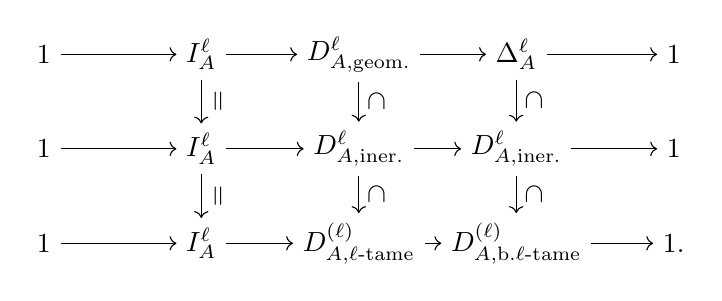
\begin{tikzpicture}[auto]
        \node (A1) at (0, 2.4) {$1$};
        \node (B1) at (0, 1.2) {$1$};
        \node (C1) at (0, 0) {$1$};
        \node (A2) at (2.0, 2.4) {$\PRIG{\ell}{A}$};
        \node (B2) at (2.0, 1.2) {$\PRIG{\ell}{A}$};
        \node (C2) at (2.0, 0) {$\PRIG{\ell}{A}$};
        \node (A3) at (4.0, 2.4) {$\GPRDG{\ell}{A}$};
        \node (B3) at (4.0, 1.2) {$\IPRDG{\ell}{A}$};
        \node (C3) at (4.0, 0) {$\lTRGPRDG{\ell}{A}$};
        \node (A4) at (6.0, 2.4) {$\GFG{A}^\ell$};
        \node (B4) at (6.0, 1.2) {$\IPRDG{\ell}{A}$};
        \node (C4) at (6.0, 0) {$\lTRGPRBDG{\ell}{A}$};
        \node (A5) at (8.0, 2.4) {$1$};
        \node (B5) at (8.0, 1.2) {$1$};
        \node (C5) at (8.0, 0) {$1.$};
        \draw[->] (A1) to node {} (A2);
        \draw[->] (B1) to node {} (B2);
        \draw[->] (C1) to node {} (C2);
        \draw[->] (A2) to node {} (A3);
        \draw[->] (B2) to node {} (B3);
        \draw[->] (C2) to node {} (C3);
        \draw[->] (A3) to node {} (A4);
        \draw[->] (B3) to node {} (B4);
        \draw[->] (C3) to node {} (C4);
        \draw[->] (A4) to node {} (A5);
        \draw[->] (B4) to node {} (B5);
        \draw[->] (C4) to node {} (C5);
        \draw[->] (A2) to node {\rotatebox{270}{$=$}} (B2);
        \draw[->] (B2) to node {\rotatebox{270}{$=$}} (C2);
        \draw[->] (A3) to node {\rotatebox{270}{$\subset$}} (B3);
        \draw[->] (B3) to node {\rotatebox{270}{$\subset$}} (C3);
        \draw[->] (A4) to node {\rotatebox{270}{$\subset$}} (B4);
        \draw[->] (B4) to node {\rotatebox{270}{$\subset$}} (C4);
      \end{tikzpicture}
    \end{center}
    Then all the horizontal sequences in the diagram are exact.
    \item Assume that $\sign{\eta_A}(0) = \textS$. Now we consider the (natural) commutative diagram of profinite groups
    \begin{center}
      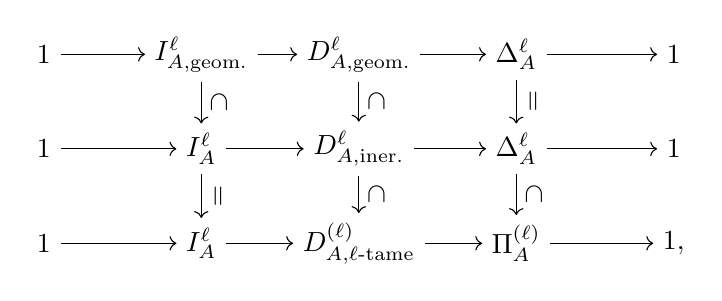
\begin{tikzpicture}[auto]
        \node (A1) at (0, 2.4) {$1$};
        \node (B1) at (0, 1.2) {$1$};
        \node (C1) at (0, 0) {$1$};
        \node (A2) at (2.0, 2.4) {$\GPRIG{\ell}{A}$};
        \node (B2) at (2.0, 1.2) {$\PRIG{\ell}{A}$};
        \node (C2) at (2.0, 0) {$\PRIG{\ell}{A}$};
        \node (A3) at (4.0, 2.4) {$\GPRDG{\ell}{A}$};
        \node (B3) at (4.0, 1.2) {$\IPRDG{\ell}{A}$};
        \node (C3) at (4.0, 0) {$\lTRGPRDG{\ell}{A}$};
        \node (A4) at (6.0, 2.4) {$\GFG{A}^\ell$};
        \node (B4) at (6.0, 1.2) {$\GFG{A}^\ell$};
        \node (C4) at (6.0, 0) {$\GPRFG{\ell}{A}$};
        \node (A5) at (8.0, 2.4) {$1$};
        \node (B5) at (8.0, 1.2) {$1$};
        \node (C5) at (8.0, 0) {$1,$};
        \draw[->] (A1) to node {} (A2);
        \draw[->] (B1) to node {} (B2);
        \draw[->] (C1) to node {} (C2);
        \draw[->] (A2) to node {} (A3);
        \draw[->] (B2) to node {} (B3);
        \draw[->] (C2) to node {} (C3);
        \draw[->] (A3) to node {} (A4);
        \draw[->] (B3) to node {} (B4);
        \draw[->] (C3) to node {} (C4);
        \draw[->] (A4) to node {} (A5);
        \draw[->] (B4) to node {} (B5);
        \draw[->] (C4) to node {} (C5);
        \draw[->] (A2) to node {\rotatebox{270}{$\subset$}} (B2);
        \draw[->] (B2) to node {\rotatebox{270}{$=$}} (C2);
        \draw[->] (A3) to node {\rotatebox{270}{$\subset$}} (B3);
        \draw[->] (B3) to node {\rotatebox{270}{$\subset$}} (C3);
        \draw[->] (A4) to node {\rotatebox{270}{$=$}} (B4);
        \draw[->] (B4) to node {\rotatebox{270}{$\subset$}} (C4);
      \end{tikzpicture}
    \end{center}
    where $\GPRFG{\ell}{A}$ is the geometrically pro-$\ell$ fundamental group of $A$. Then all the horizontal sequences in the diagram are exact.
    \item Assume that $\sign{\eta_A}(n) = \textV$ (respectively, $\sign{\eta_A}(n) = \textC$; $\sign{\eta_A}(n) = \textN$). Let $A_\text{fib.}^\log$ be the log geometric fiber $A^\log \times_{\overline{A}^\log} \overline{a}^\log$. Then the natural sequence of profinite groups
    \[
      1 \to \pi_1(A_\text{fib.}^\log, a^\log)^\ell \to \GPRDG{\ell}{A} \to \GPRDG{\ell}{\overline{A}} \to 1,
    \]
    is exact.
    \item In the notation of (iv), write $\GFG{X_n/X_{n - 1}}^\ell$ for the kernel of the natural morphism $\GFG{X_n}^\ell \to \GFG{X_{n - 1}}^\ell$. By the assertion (i) above, we can obtain the natural morphism of profinite groups $\pi_1(A_\text{fib.}^\log, a^\log)^\ell \to \GFG{X_n/X_{n - 1}}^\ell$. Then the morphism $\pi_1(A_\text{fib.}^\log, a^\log)^\ell \to \GFG{X_n/X_{n - 1}}^\ell$ is injective. Moreover, the image of the morphism $\pi_1(A_\text{fib.}^\log, a^\log)^\ell \to \GFG{X_n/X_{n - 1}}^\ell$ is a verticial subgroup (respectively, a cuspidal subgroup; a nodal subgroup) of $\GFG{X_n/X_{n - 1}}^\ell$, where we identify $\GFG{X_n/X_{n - 1}}^\ell$ with the [log geometric] pro-$\ell$ fundamental group of the log stable curve $\model{X}^\log_n \times_{\model{X}^\log_{n - 1}} \overline{a}^\log$ over the log geometric point $\overline{a}^\log$.
    \item Let $r$ be the log-rank of $A^\log$. The pro-$\ell$ inertia group $\PRIG{\ell}{A}$ of $A$ is a free $\Int_\ell$-module of rank $r$. Moreover, with respect to the natural action of $\pi_1(A, a)$ on $\PRIG{\ell}{A}$, the pro-$\ell$ inertia group $\PRIG{\ell}{A}$ is isomorphic to the $r$-fold direct product of the pro-$\ell$ cyclotomes $\Int_\ell(1)$.
    \item Assume that $\sign{\eta_A}(0) = \textS$. Then the geometric pro-$\ell$ inertia group $\GPRIG{\ell}{A}$ is a free $\Int_\ell$-module of rank $r - 1$, where $r$ is the log-rank of $A^\log$.
    \item We identify $\PRIG{\ell}{A}$ with its image in $\IPRDG{\ell}{A}$ via the injective morphism described above. Then the equality $C(\IPRDG{\ell}{A}) = \PRIG{\ell}{A}$ holds.
  \end{enumerate}
\end{prop}
\begin{proof}
  We verify assertions (i), (ii), (iii), (iv), and (v) simultaneously by induction on $n$. The case where $n = 0$ is trivial. Assume that $n > 0$ and that the assertions hold for smaller values of $n$.

  We first observe, in light of the definition of the stratification, that the morphism $A^\log \to \overline{A}^\log$ is a hyperbolic curve over $\overline{A}^\log$ if $\sign{\eta_A}(n) = \textV$. Moreover, in that case, there is a compactification $A^\log_\cpt$ of $A^\log$ as a hyperbolic curve which is obtained as an irreducible component of $\model{X}^\log_n \times_{\model{X}^\log_{n - 1}} \overline{A}^\log$.
\end{proof}





% #endregion




% チェックポイント: strata vs. stratum 問題, complete うまくいってるか問題, cusp 忘れてないか問題, 概念の名前だいじょうぶか問題, Notation check,



\newpage
\section{Cofinality of $l$-admissible finite \'{e}tale coverings}

\begin{defn}
  Let $K$ be a field and $X = X_n \to X_{n - 1} \to \cdots \to X_1 \to X_0 = \Spec \, K$ a hyperbolic polycurve over $K$. We shall say that $X$ is \emph{pro-$l$ exact} (with respect to its parametrization) if for each $0 \leq i \leq n$, the (natural) sequence of profinite groups \[ 1 \to \GFG{X_n/X_i}^l \to \FG{X_n}^l \to \FG{X_i}^l \to 1 \] is exact. Here, $\GFG{X_n/X_i}$ denotes the kernel of the homomorphism $\FG{X_n} \to \FG{X_i}$ induced by the morphism $X_n \to X_i$.
\end{defn}

\begin{defn}
  Let $K$ be a valuation field and $X = X_n \to X_{n - 1} \to \cdots \to X_1 \to X_0 = \Spec \, K$ a hyperbolic polycurve over $K$. Let $l$ be a prime number which is different from the characteristic of the residue field of $K$. We shall say that $X$ is \emph{$l$-quasi-fine} (with respect to its parametrization) if $X$ admits a compactified stable model $\model{X} = \model{X}_n \to \model{X}_{n - 1} \to \cdots \to \model{X}_1 \to \model{X}_0 = \Spec \, \mathcal{O}_K$ and $X$ is pro-$l$ exact. We shall say that $X$ is \emph{$l$-fine} (with respect to its parametrization) if $X$ is $l$-quasi-fine and for each $i = 1, \ldots, n$ and each geometric point $\overline{x}$ of $X_{i - 1}$ which lies over the closed point of $\Spec \, \mathcal{O}_K$, the geometric fiber $X_{i, \overline{x}}$ of the morphism $X_i \to X_{i - 1}$ over $\overline{x}$ is singular. 
\end{defn}

\begin{thm}
  Let $K$ be a valuation field and $X = X_n \to X_{n - 1} \to \cdots \to X_1 \to X_0 = \Spec \, K$ a hyperbolic polycurve over $K$. Let $l$ be a prime number which is different from the characteristic of the residue field of $K$. Then there exists a finite \'{e}tale covering $Y \to X$ such that $Y$ is $l$-fine (with respect to its parametrization induced by the morphism $Y \to X$).
\end{thm}
\begin{proof}
  proof here
\end{proof}

\newpage
\section{Dehn-twist Pointed Stable Curves type Outer Representations}
\indent In this section, first, we review the basic theory of profinite Dehn multi-twists (cf. \cite[\S 4]{CbTpI}). We then introduce the notion of Dehn-twist pointed stable curves type outer representations as a certain generalization of IPSC-type [cf. \cite[Definition 2.4, (i)]{NodNon}] and SNN-type [cf. \cite[Definition 2.4, (iii)]{NodNon}] outer representations, and investigate their basic properties. Finally, we investigate the natural outer representations of semi-graph of anabelioids associated to the strata defined in the previous section, and in particular verify that the outer representations of inertia groups are of Dehn-twist pointed stable curves type.

\begin{defn}
  Let $\Sigma$ be a nonempty set of prime numbers, and let $\Gcal$ be a semi-graph of anabelioids of pro-$\Sigma$ PSC-type. Write $\univG \to \Gcal$ for the universal [pro-]covering of $\Gcal$ corresponding to $\PiG$. Then we shall write
  \[
    \Dehn{\Gcal} \coloneqq \{ \alpha \in \Aut^{|\text{grph}|}(\Gcal) \mid \alpha_{\Gcal|_v} = \mathrm{id}_{\Gcal|_v} \text{ for any } v \in v(\Gcal) \}
  \]
  --- where we refer to \cite[Definition 2.1, (iii)]{CbTpI}, \cite[Definition 2.14, (ii)]{CbTpI}, \cite[Remark 2.5.1]{CbTpI}. We shall refer to an element of $\Dehn{\Gcal}$ as a \emph{profinite Dehn multi-twist} of $\Gcal$.
\end{defn}

\begin{defn}\label{SignedNodalGroup}
  Let $\Sigma$ be a nonempty set of prime numbers, and let $\Gcal$ be a semi-graph of anabelioids of pro-$\Sigma$ PSC-type. Write $\univG \to \Gcal$ for the universal [pro-]covering of $\Gcal$ corresponding to $\PiG$. Let $\univ{e} \in \Node{\univG}$, $e \coloneqq \univ{e}(\Gcal) \in \Node{\Gcal}$. Write $\univ{v_1}, \univ{v_2} \in \Vcal(\univ{e})$ for the two vertices of $\univG$ adjacent to $\univ{e}$. Let $M_1, M_2 \coloneqq \Pi_{\univ{e}}$ (respectively, $N_1, N_2 \coloneqq \Pi_e$). Write $\Delta_M$ (respectively, $\Delta_N$) be the image of the ``diagonal'' embedding $\Pi_{\univ{e}} \to M_1 \times M_2$; $x \mapsto (x, x)$ (respectively, $\Pi_e \to N_1 \times N_2$; $x \mapsto (x, x)$). We shall refer to $M_1 \times M_2 / \Delta_M$ (respectively, $N_1 \times N_2 / \Delta_N$) as the \emph{signed nodal group} associated to $\univ{e}$ (respectively, $e$), and denote it by $\sgnnodal{\univ{e}}$ (respectively, $\sgnnodal{e}$). Let $x \in \Pi_{\univ{e}}$ (respectively, $x \in \Pi_e$). We shall denote the image of $(x, 1) \in M_1 \times M_2$ (respectively, $(x, 1) \in N_1 \times N_2$) in $\sgnnodal{\univ{e}}$ (respectively, $\sgnnodal{e}$) by $[x, \univ{v_1}]$ (respectively, $[x, v_1]$), and the image of $(1, x) \in M_1 \times M_2$ (respectively, $(1, x) \in N_1 \times N_2$) in $\sgnnodal{\univ{e}}$ (respectively, $\sgnnodal{e}$) by $[x, \univ{v_2}]$ (respectively, $[x, v_2]$).
\end{defn}

\begin{rem}
  In the notation of Definition \ref{SignedNodalGroup}, the signed nodal group $\sgnnodal{\univ{e}}$ associated to $\univ{e}$ can be naturally identified with the signed nodal group $\sgnnodal{e}$ associated to $e$.
\end{rem}

\begin{defn}
  Let $\Sigma$ be a nonempty set of prime numbers, and let $\Gcal$ be a semi-graph of anabelioids of pro-$\Sigma$ PSC-type. Let $\alpha \in \Dehn{\Gcal}$ be a profinite Dehn multi-twist of $\Gcal$. Let $\univ{e} \in \Node{\univG}$, $e \coloneqq \univ{e}(\Gcal) \in \Node{\Gcal}$. We define an element of $\sgnnodal{\univ{e}}$ as follows.
  \begin{itemize}
  \item Let $\univ{v} \in \Vcal(\univ{e})$. Then there exists a unique lifting $\alpha[\univ{v}] \in \Aut(\PiG)$ of $\alpha$ such that $\alpha$ preserves $\Pi_{\univ{v}}$ and induces the identity on $\Pi_{\univ{v}}$. Here, letting $\univ{w} \in \Vcal(\univ{e})$ be the other vertex of $\univG$ adjacent to $\univ{e}$, $\alpha$ induces an inner automorphism of $\Pi_{\univ{w}}$. Therefore, there exists a unique element $\delta_{\alpha, \univ{v}} \in \Pi_{\univ{e}}$ such that $\alpha[\univ{v}]|_{\Pi_{\univ{w}}}$ coincides with the inner automorphism of $\Pi_{\univ{w}}$ arising from the conjugation action of $\delta_{\alpha, \univ{v}}$. We shall denote the element $[\delta_{\alpha, \univ{v}}, \univ{v}]$ of $\sgnnodal{\univ{e}}$ by $\delta_{\alpha, \univ{e}}$.
  \end{itemize}
  We note, in light of \cite[Lemma 4.6]{CbTpI}, that this definition is well-defined. We denote the morphism $\Dehn{\Gcal} \to \sgnnodal{\univ{e}}$ given by assigning $\alpha \mapsto \delta_{\alpha, \univ{e}}$ by $\Dpar{\univ{e}}$.
\end{defn}

\begin{lem}
  Let $\Sigma$ be a nonempty set of prime numbers, and let $\Gcal$ be a semi-graph of anabelioids of pro-$\Sigma$ PSC-type. Let $\univ{e} \in \Node{\univG}$, $e \coloneqq \univ{e}(\Gcal) \in \Node{\Gcal}$. Then the following hold.
  \begin{enumerate}
    \item
    \item
  \end{enumerate}
\end{lem}
\begin{proof}
  
\end{proof}

\begin{defn}
  DTPSC-type outer representation, 退化している node
\end{defn}

\begin{lem}
  center とかの群論の計算、inertia の話
\end{lem}
\begin{proof}
  NodNon など
\end{proof}


inertia の線形代数は、かかないといけない

あとは、strata に付随する外表現 (環論との対応)

\newpage
\section{Reconstruction of Log-full Subgroups}
「$l$-fine な polycurve が与えられたなら、[HMM] の議論をそのまま援用することで、residually $l$-cyclotomicaly full くらいの状況のもとで、log full subgroup を思い出すことができる。ほとんど議論一緒なのでアレだけど、self-contained-ness のこともあって、もう一度かいてみる。ただし、本質的に新しいことはなにもしていないことには注意したい。」

\newpage
\section{Reconstruction of Dimensions via Corank 1 Intersections}
\input{CorankOneIntersections.tex}

\newpage
\section{Reconstruction of the Graph-theoretic Structure of Proper Hyperbolic Polycurves of Dimension 2}
\input{GraphStructure.tex}

\newpage
\section*{References}
% EP, MT, Hur, KatoF

\begin{thebibliography}{99999999}
\bibitem[KatoF]{KatoF} F.~Kato, \textit{Log smooth deformation and moduli of log smooth curves}, Int. J. Math. \textbf{11} (2000), no. 2, 215–-232.

\bibitem[MT]{MT} S.~Mochizuki and A.~Tamagawa, \textit{The algebraic and anableian geometry of configuration spaces}, Hokkaido Math. J. \textbf{37} (2008), 75--131.

\bibitem[DM]{DM} P.~Deligne and D.~Mumford, \textit{The irreducibility of the space of curves of given genus}, IHES Publ. Math. \textbf{36} (1969), 75--109.

\bibitem[Hur]{Hur} S.~Mochizuki, \textit{The geometry of the compactification of the Hurwitz scheme}, Publ. Res. Inst. Math. Sci. \textbf{31} (1995), 355--441.

\bibitem[CmbGC]{CmbGC} S.~Mochizuki, \textit{A combinatorial version of the Grothendieck conjecture}, Tohoku Math. J. \textbf{59} (2007), 455--479.

\bibitem[CbGT]{CbGT} Y.~Hoshi, A.~Minamide, and S.~Mochizuki, \textit{Group-theoreticity of numerical invariants and distinguished subgroups of configuration space groups}, Kodai Math. J. \textbf{45} (2022), 295--348.

\bibitem[NodNon]{NodNon} Y.~Hoshi and S.~Mochizuki, \textit{On the combinatorial anabelian geometry of nodally nondegenerate outer representations}, Hiroshima Math. J. \textbf{41} (2011), 275--342.

\bibitem[CbTpI]{CbTpI} Y.~Hoshi and S.~Mochizuki, \textit{Topics surrounding the combinatorial anabelian geometry of hyperbolic curves I: Inertia groups and profinite Dehn twists}, Galois-Teichm\"{u}ller Theory and Arithmetic Geometry, Adv. Stud. Pure Math., \textbf{63}, Math. Soc. Japan (2012), 659--811.

\bibitem[Hoshi1]{Hoshi1} Y.~Hoshi, \textit{The exactness of the log homotopy sequence}, Hiroshima Math. J. \textbf{39} (2009), 61--121.

\bibitem[Vidal]{Vidal} I.~Vidal, \textit{Morphismes log \'{e}tales et descents par hom\'{e}omorphismes universels}, C. R. Math. Acad. Sci. Paris. \textbf{332} (2001), 239--244.

\bibitem[Kisin]{Kisin} M.~Kisin, \textit{Prime to $p$ fundamental groups and tame Galois actions}, Annals de l'Institut Fourier \textbf{50}, no. 4 (2000), 1099--1126.

\end{thebibliography}



\end{document}